\chapter{Results and Analysis}
\label{chap:results}
This chapter describes the design and results of simulations which evaluate the robustness of certain data-driven techniques.  This includes singular values (of the generalized plant), disk-based stability margins, transient responses, and integrated cost/effort metrics.  Results from the tests described in Section \ref{sect:results:testapproach} are given in the following sections.  Section \ref{sect:results:data-driven-optimal} plots the results of data-driven $\mathcal{H}_{2}$ and $\mathcal{H}_{\infty}$ optimal control.  Similar plots are provided in Section \ref{sect:results:data-driven-suboptimal}, except the data-driven $\mathcal{H}_{2}$ design uses the ``suboptimal'' performance objective described in Section \ref{sect:dataDrivenH2Suboptimal}.  Section \ref{sect:results:discussion} discusses the overall trends in the results with a focus on the effect of uncertainty, noise, and choice of performance objective.

\newpage
\section{Test Results: Data-Driven $\mathcal{H}_{2}$ and $\mathcal{H}_{\infty}$}
\label{sect:results:data-driven-optimal}
These included data-driven $\mathcal{H}_{2}$ (direct and indirect) and $\mathcal{H}_{\infty}$ (indirect).
\subsection{Parameter Uncertainty}
\subsubsection{Singular Values}
\begin{figure}[H]
\centering
	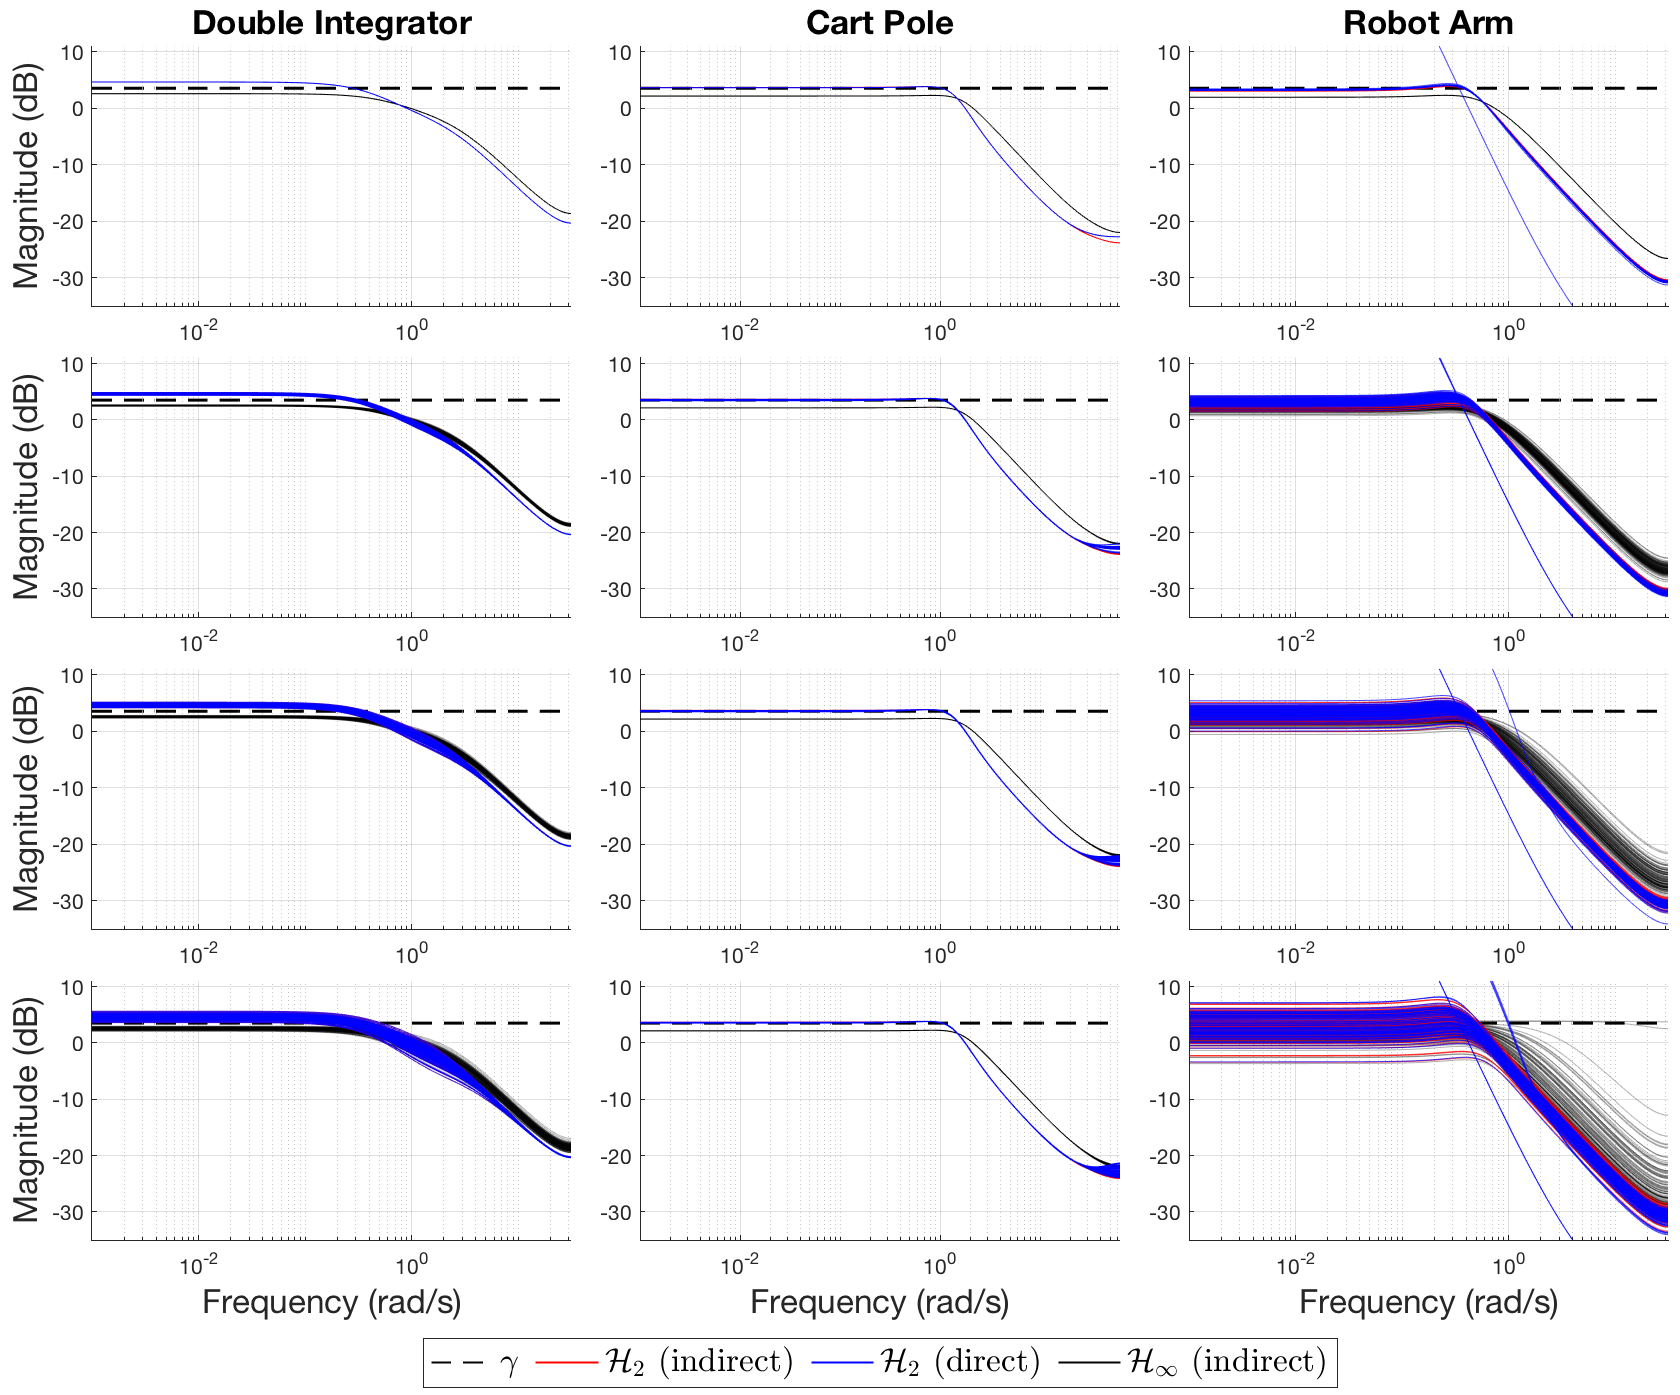
\includegraphics[width=\textwidth]{figures/uncertainty_singular_values3.png}
\caption{Maximum singular values of the closed-loop generalized plant, for controllers learned from systems with single-parameter uncertainty.  The rows correspond to respective scale factors of 0\%, 5\%, 10\%, and 20\%.  For each scale factor, the plots from 100 test runs are overlaid.}
\label{fig:uncertainty_singular_values3}
\end{figure}

\newpage
\subsubsection{Integrated Control Effort}
\begin{figure}[H]
\centering
	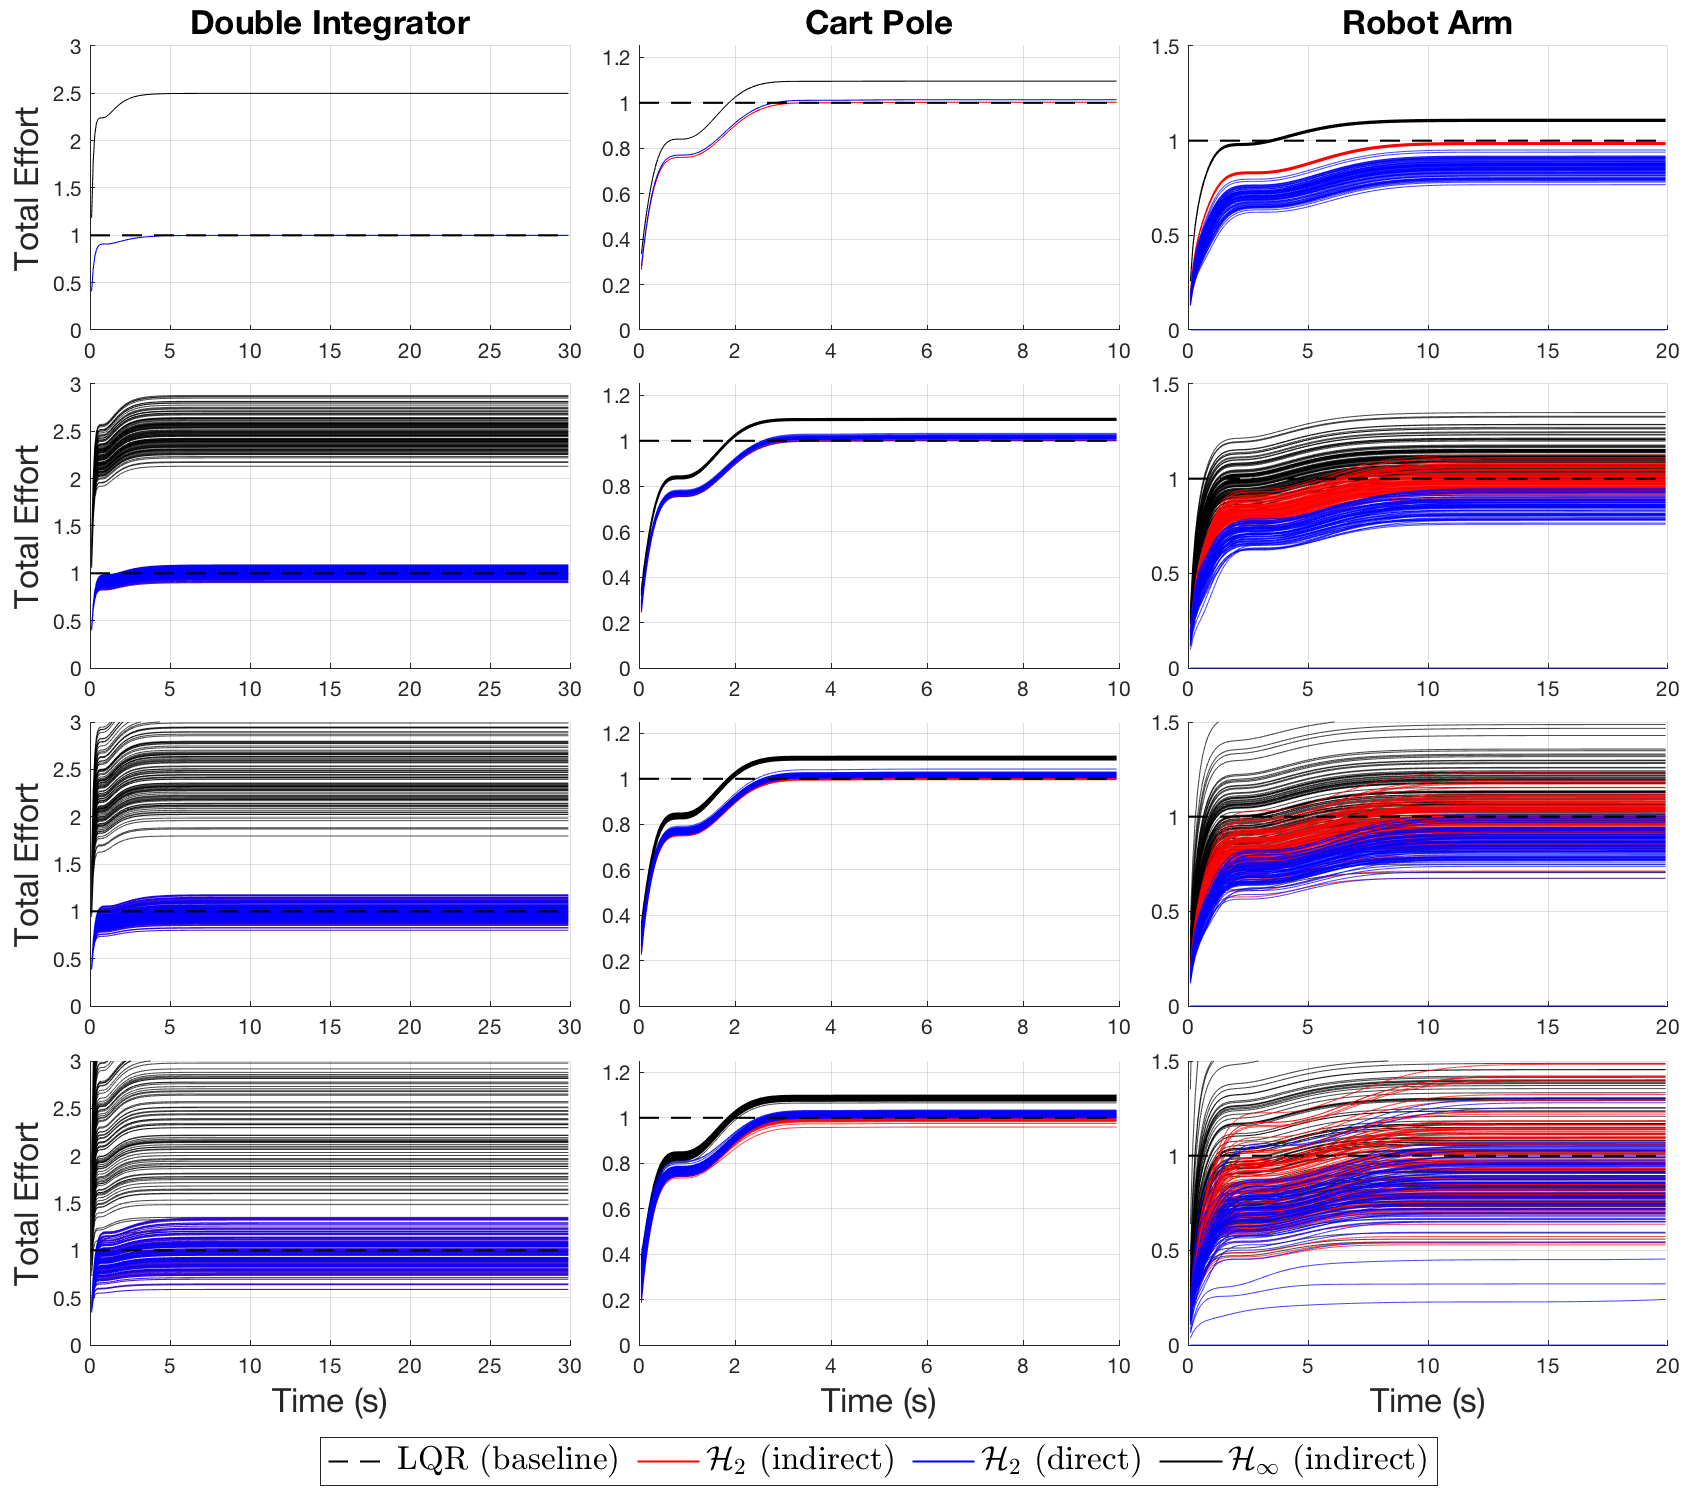
\includegraphics[width=\textwidth]{figures/uncertainty_integrated_effort3.png}
\caption{Integrated control effort of the closed-loop generalized plant, for controllers learned from systems with single-parameter uncertainty.  The rows correspond to respective scale factors of 0\%, 5\%, 10\%, and 20\%.  For each scale factor, the plots from 100 test runs are overlaid.}
\label{fig:uncertainty_integrated_effort3}
\end{figure}

\newpage
\subsubsection{Integrated LQ Cost}
\begin{figure}[H]
\centering
	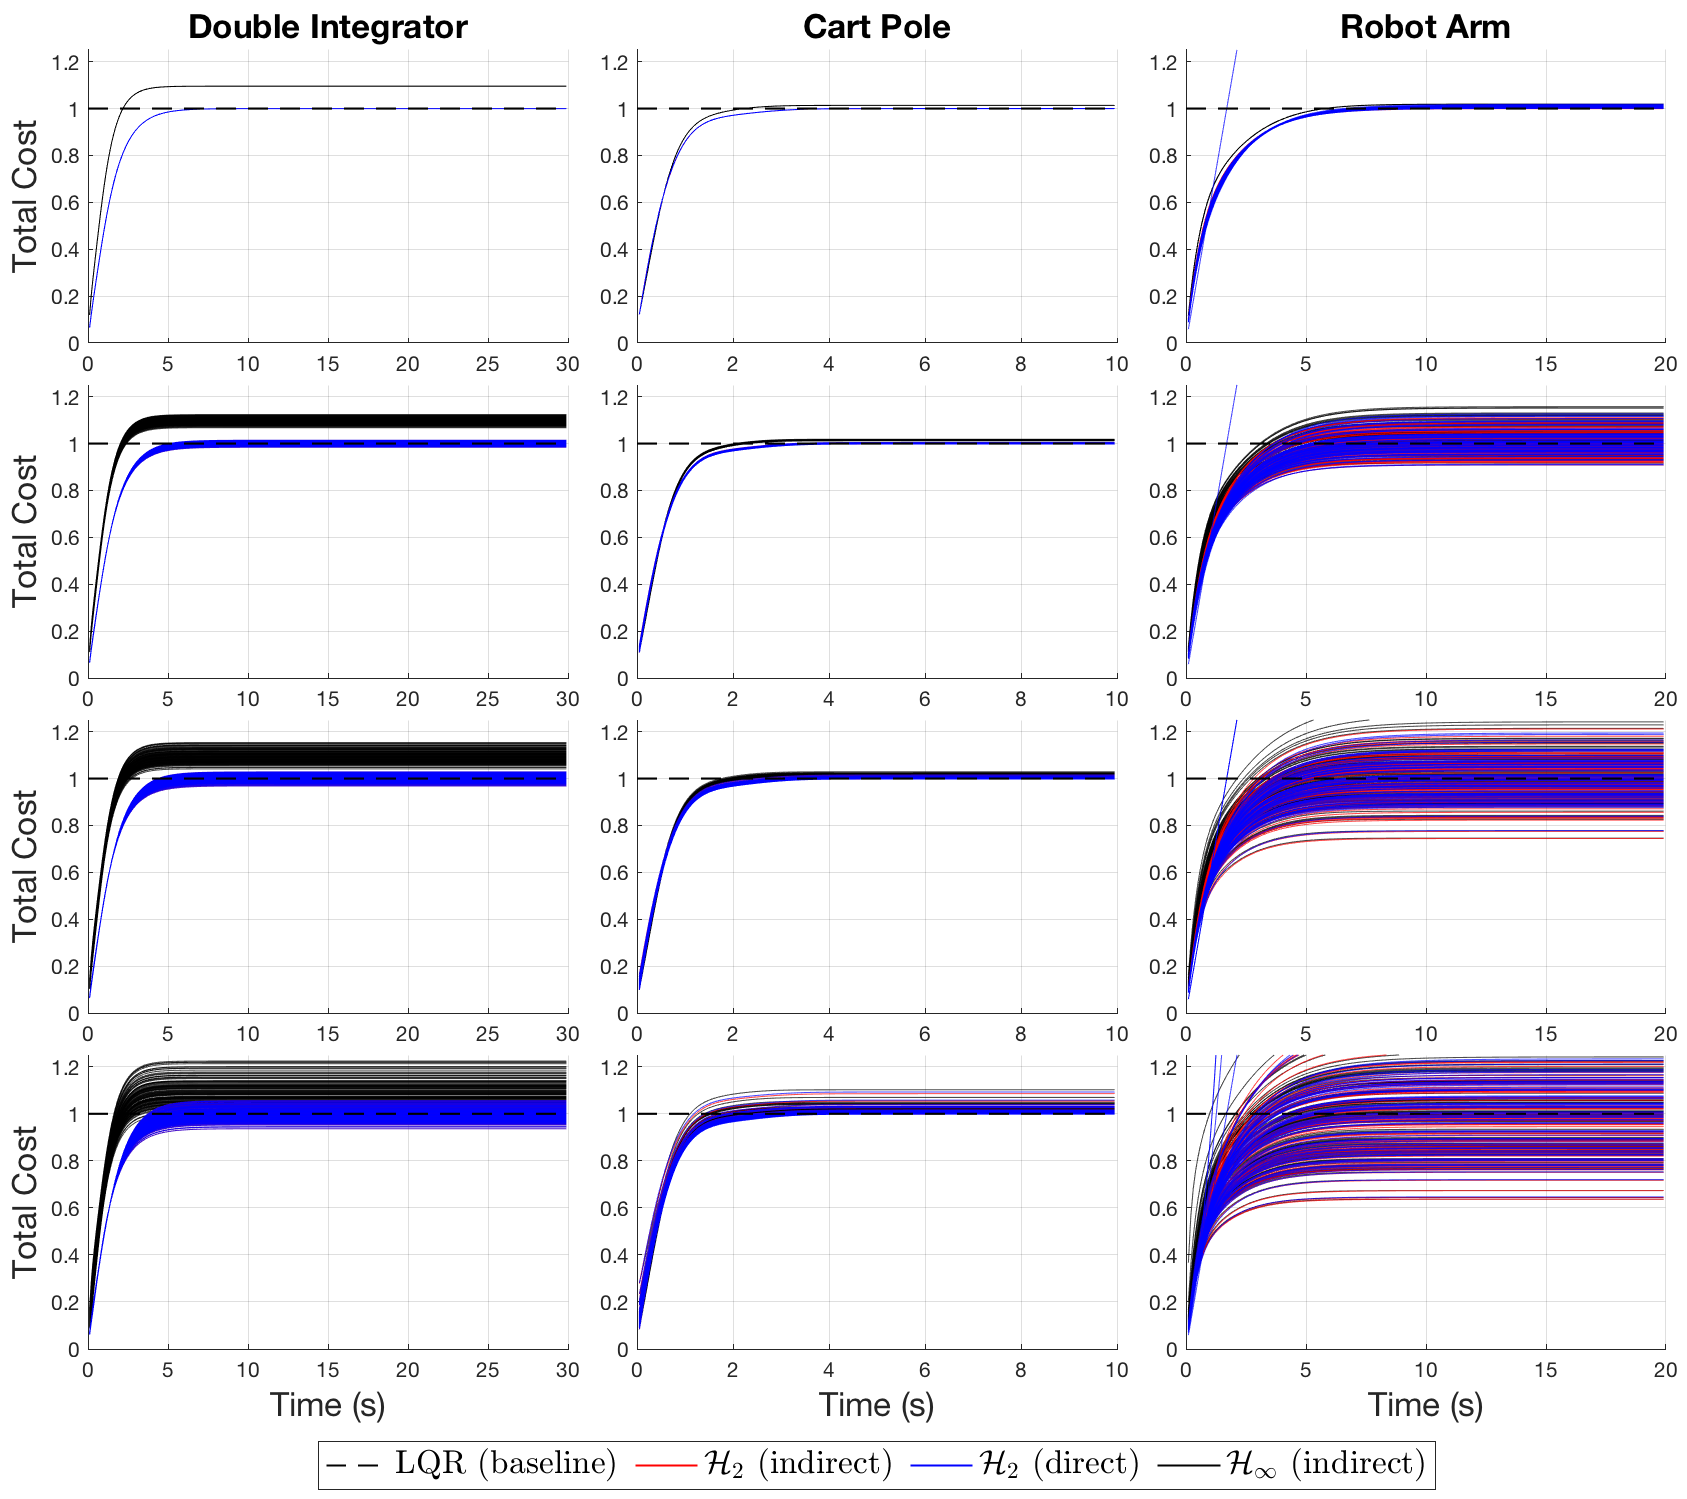
\includegraphics[width=\textwidth]{figures/uncertainty_integrated_cost3.png}
\caption{Integrated LQ cost of the closed-loop generalized plant, for controllers learned from systems with single-parameter uncertainty.  The rows correspond to respective scale factors of 0\%, 5\%, 10\%, and 20\%.  For each scale factor, the plots from 100 test runs are overlaid.}
\label{fig:uncertainty_integrated_cost3}
\end{figure}

\newpage
\subsubsection{Overall Trends}
\underline{\textbf{Note}}: Averaged metrics shown in Figure \ref{fig:overall_trends_uncertainty_opt_bar} are only defined for stable controllers, and may be skewed when the ``percent stable'' metric is significantly below 100\%.
\begin{figure}[H]
\centering
	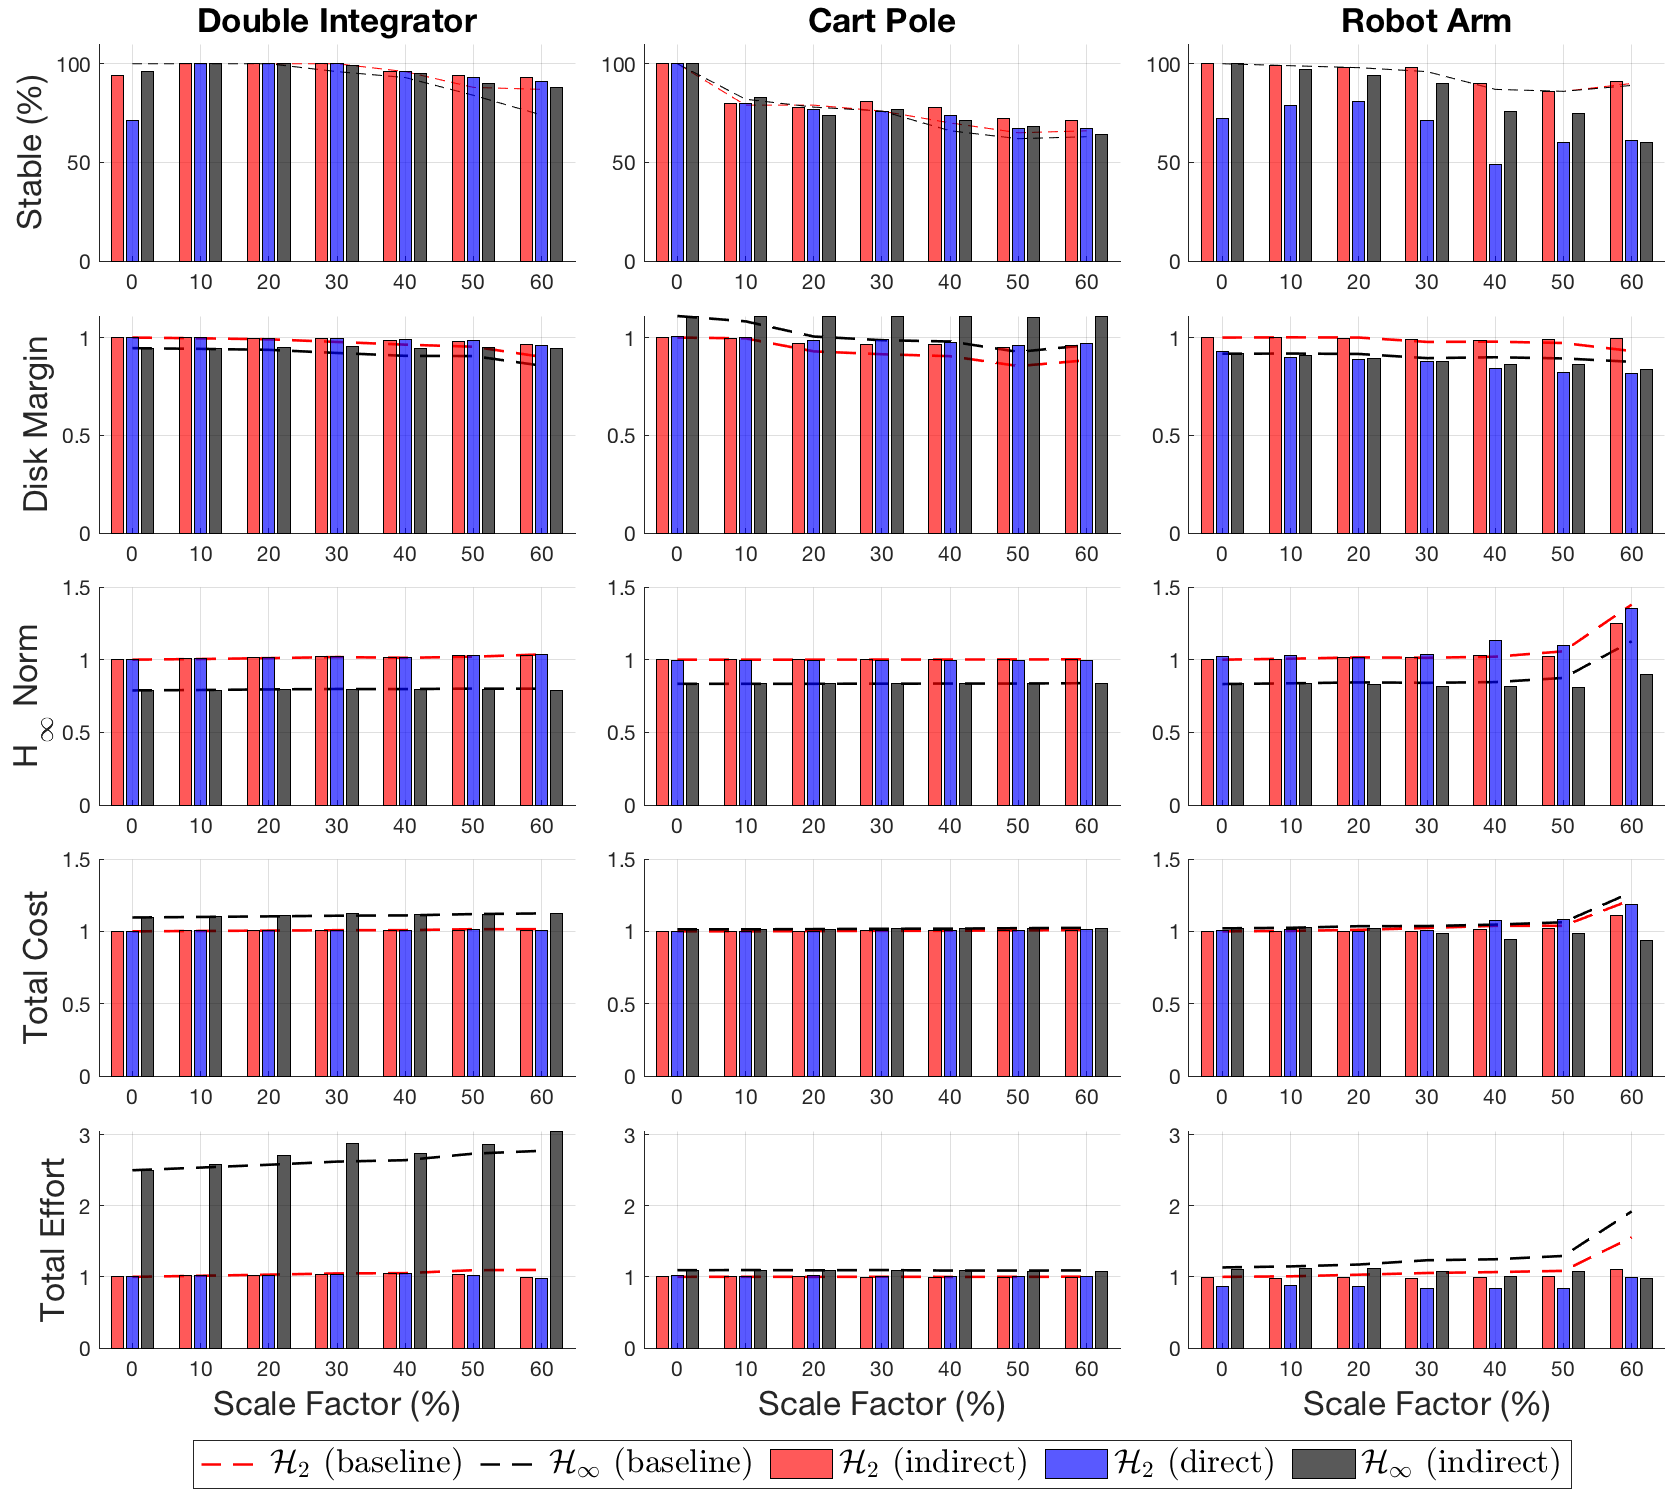
\includegraphics[width=\textwidth]{figures/overall_trends_uncertainty_opt_bar.png}
\caption{Overall trends for scaled uncertainty tests, comparing data-driven to baseline control approaches.  Apart from the percentage of stable controllers, all other metrics are normalized to what would be obtained by a nominal LQR/$\mathcal{H}_{2}$ feedback controller.  For each scale factor, the metrics shown are averaged across the stable test runs.}
\label{fig:overall_trends_uncertainty_opt_bar}
\end{figure}

\newpage
\subsection{Measurement Noise}
\subsubsection{Singular Values}
\begin{figure}[H]
\centering
	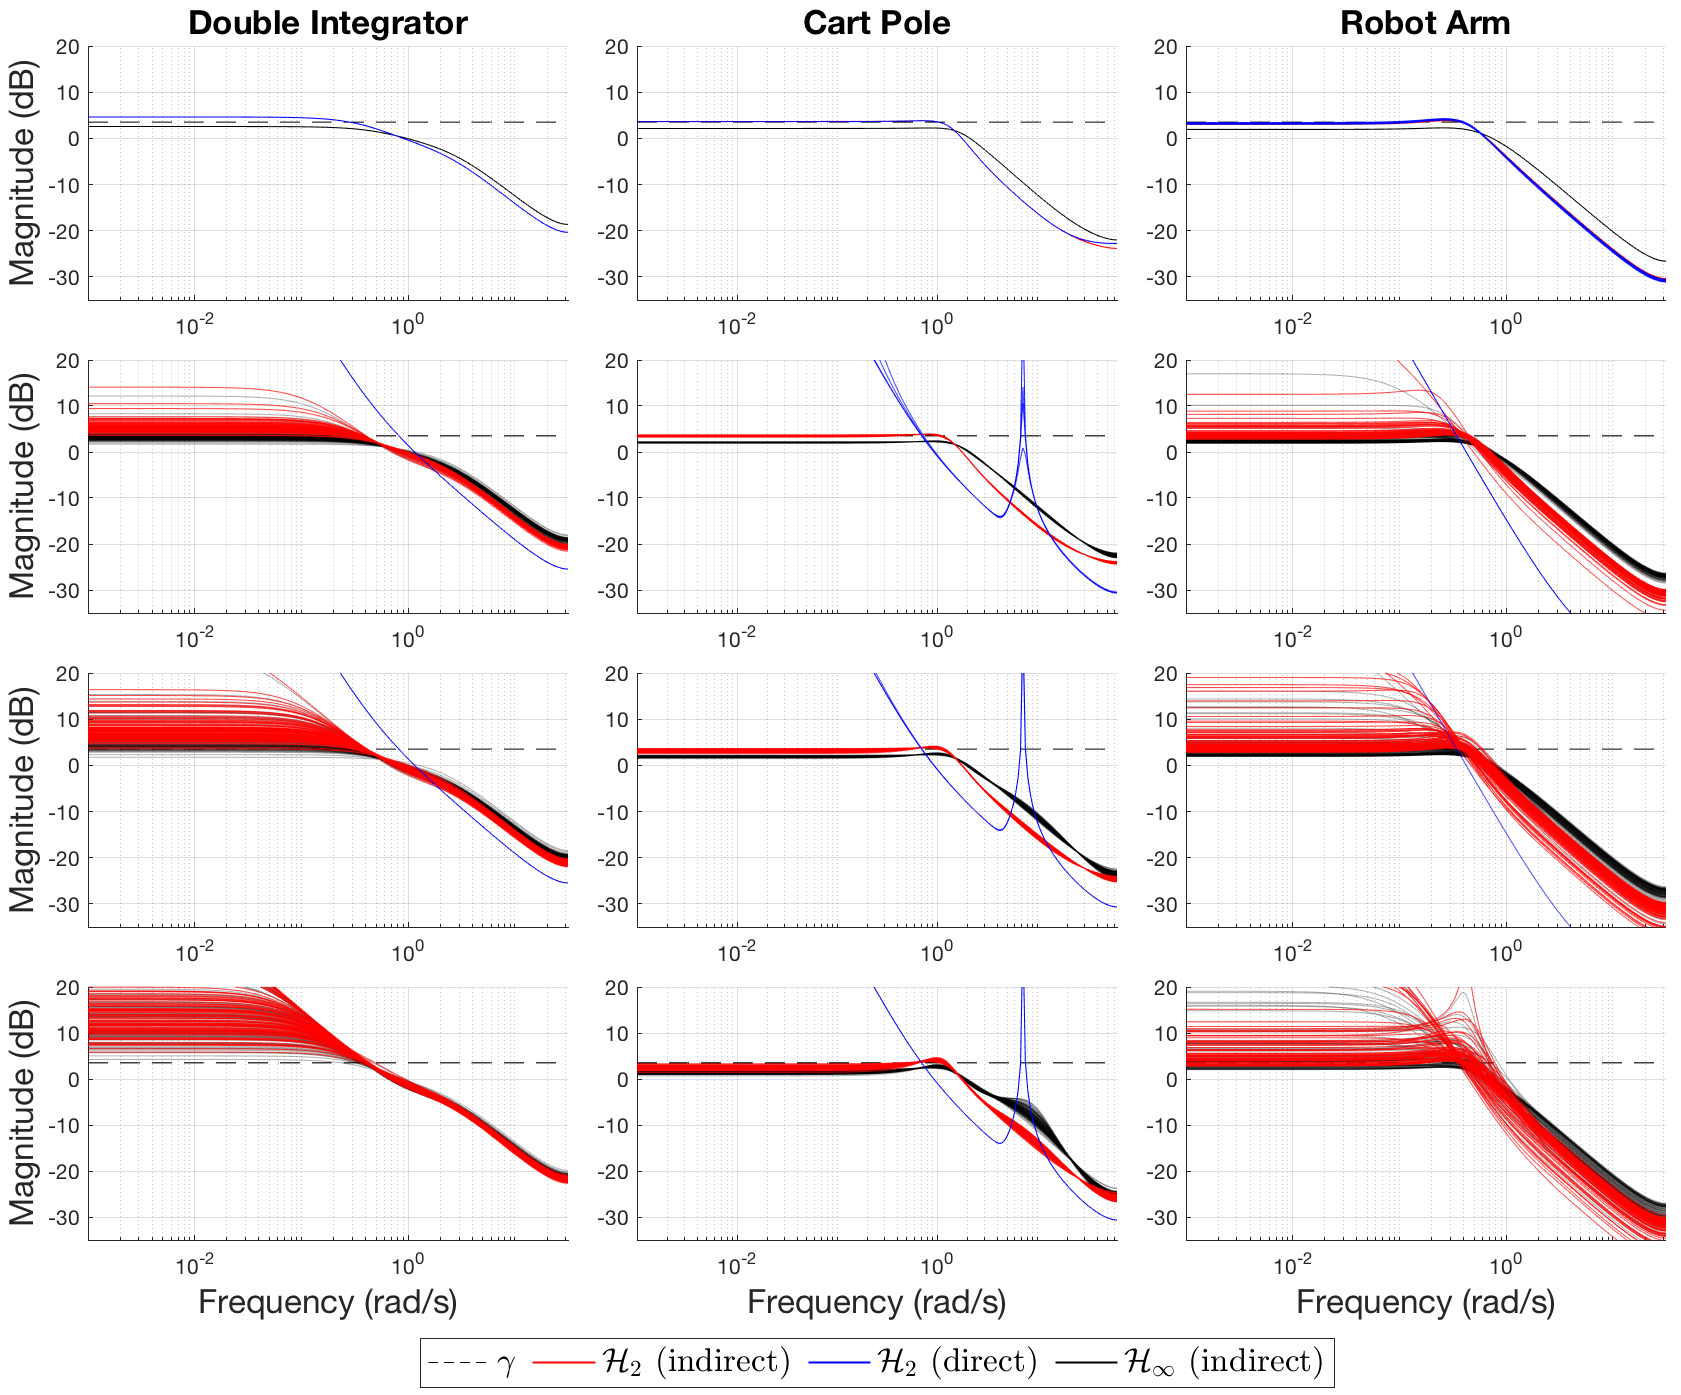
\includegraphics[width=\textwidth]{figures/noise_singular_values3.png}
\caption{Maximum singular values of the closed-loop generalized plant, for controllers learned from systems with measurement noise.  The rows correspond to respective scale factors of 0\%, 5\%, 10\%, and 20\%.  For each scale factor, the plots from 100 test runs are overlaid.}
\label{fig:noise_singular_values3}
\end{figure}

\newpage
\subsubsection{Integrated Control Effort}
\begin{figure}[H]
\centering
	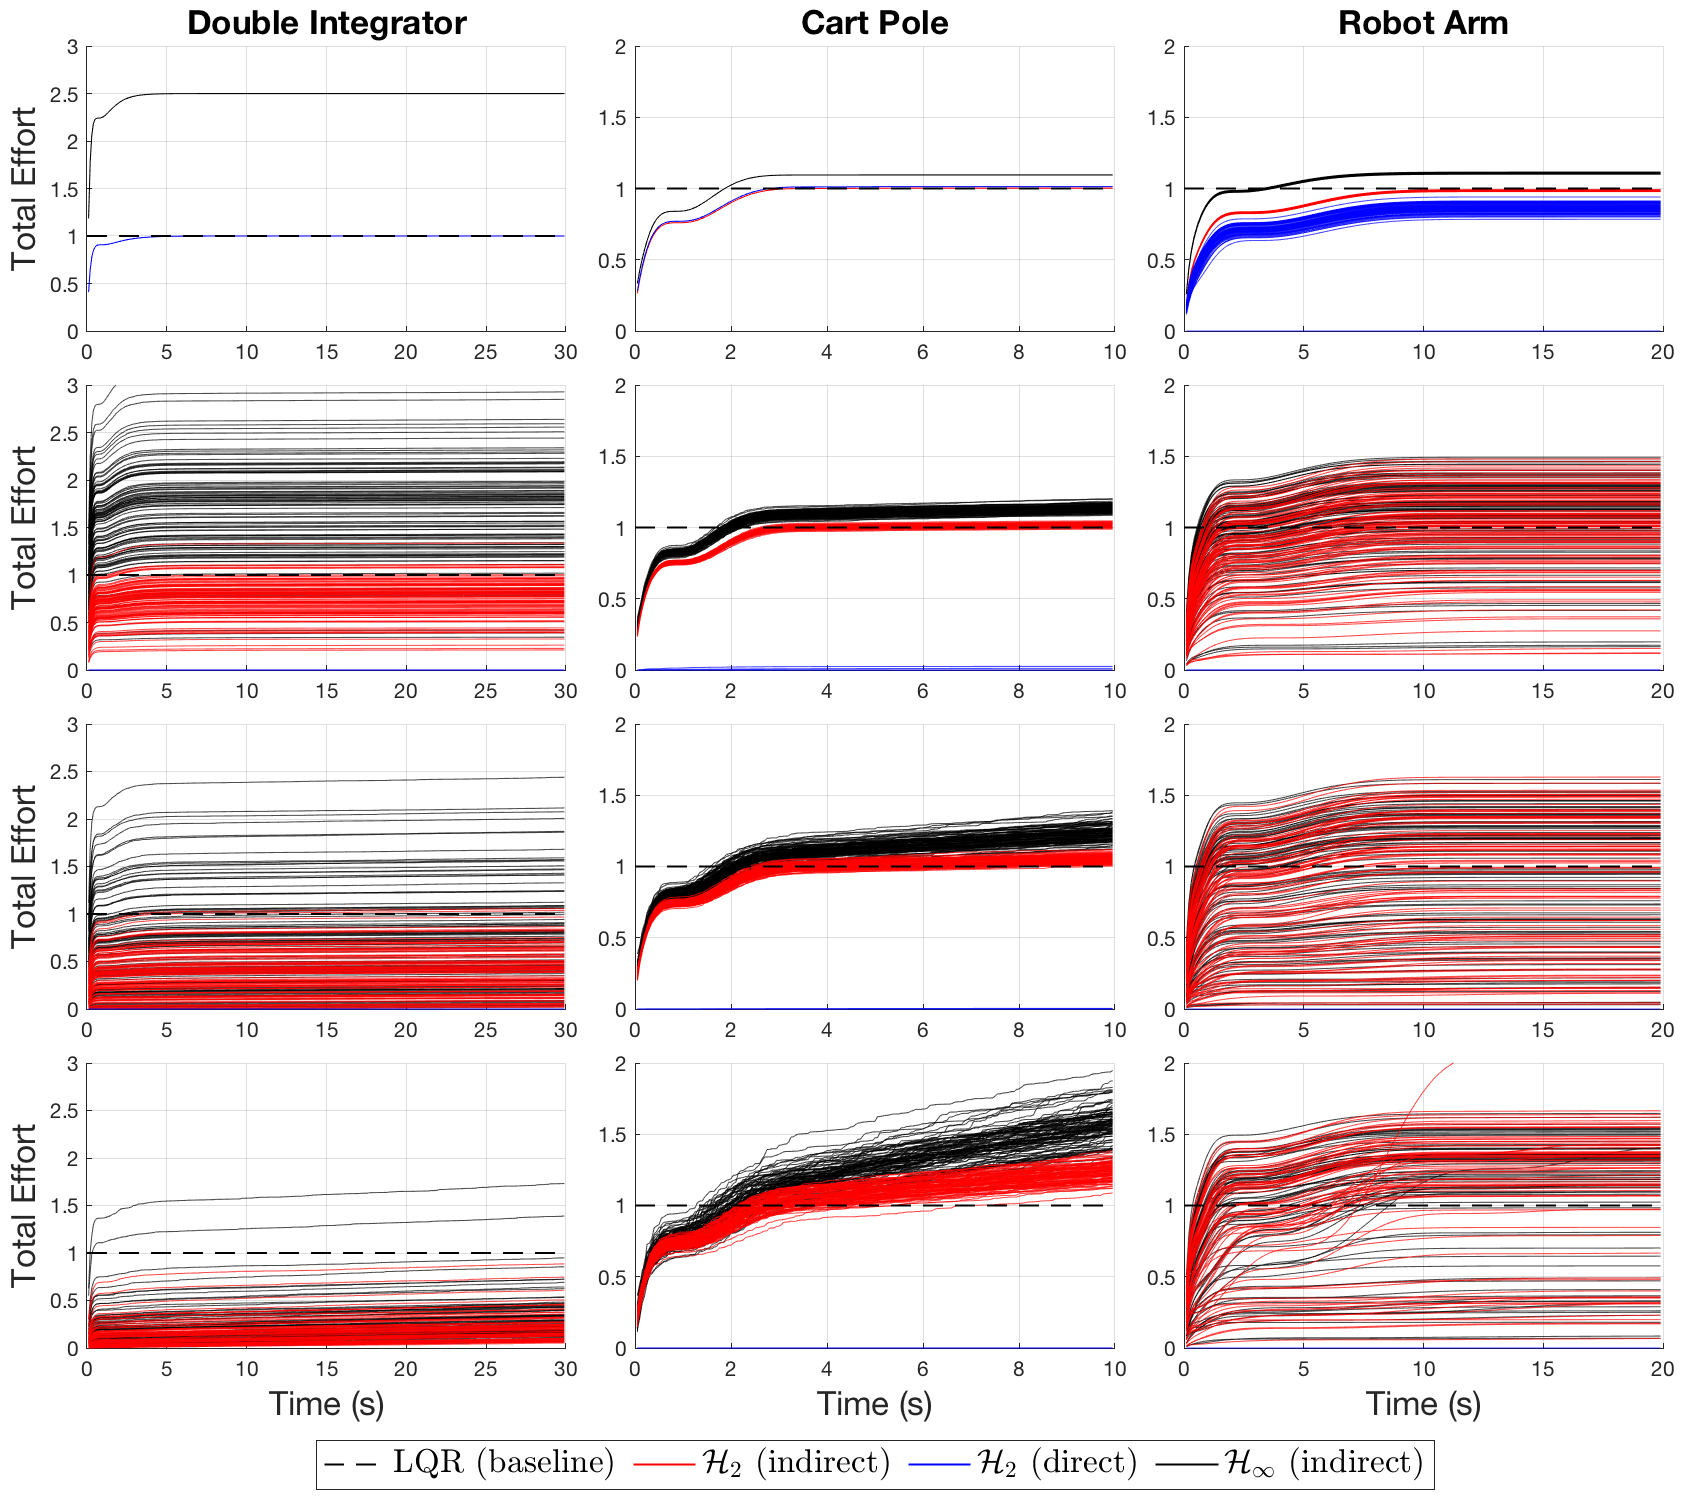
\includegraphics[width=\textwidth]{figures/noise_integrated_effort3.png}
\caption{Integrated control effort of the closed-loop generalized plant, for controllers learned from systems with measurement noise.  The rows correspond to respective scale factors of 0\%, 5\%, 10\%, and 20\%.  For each scale factor, the plots from 100 test runs are overlaid.}
\label{fig:noise_integrated_effort3}
\end{figure}

\newpage
\subsubsection{Integrated LQ Cost}
\begin{figure}[H]
\centering
	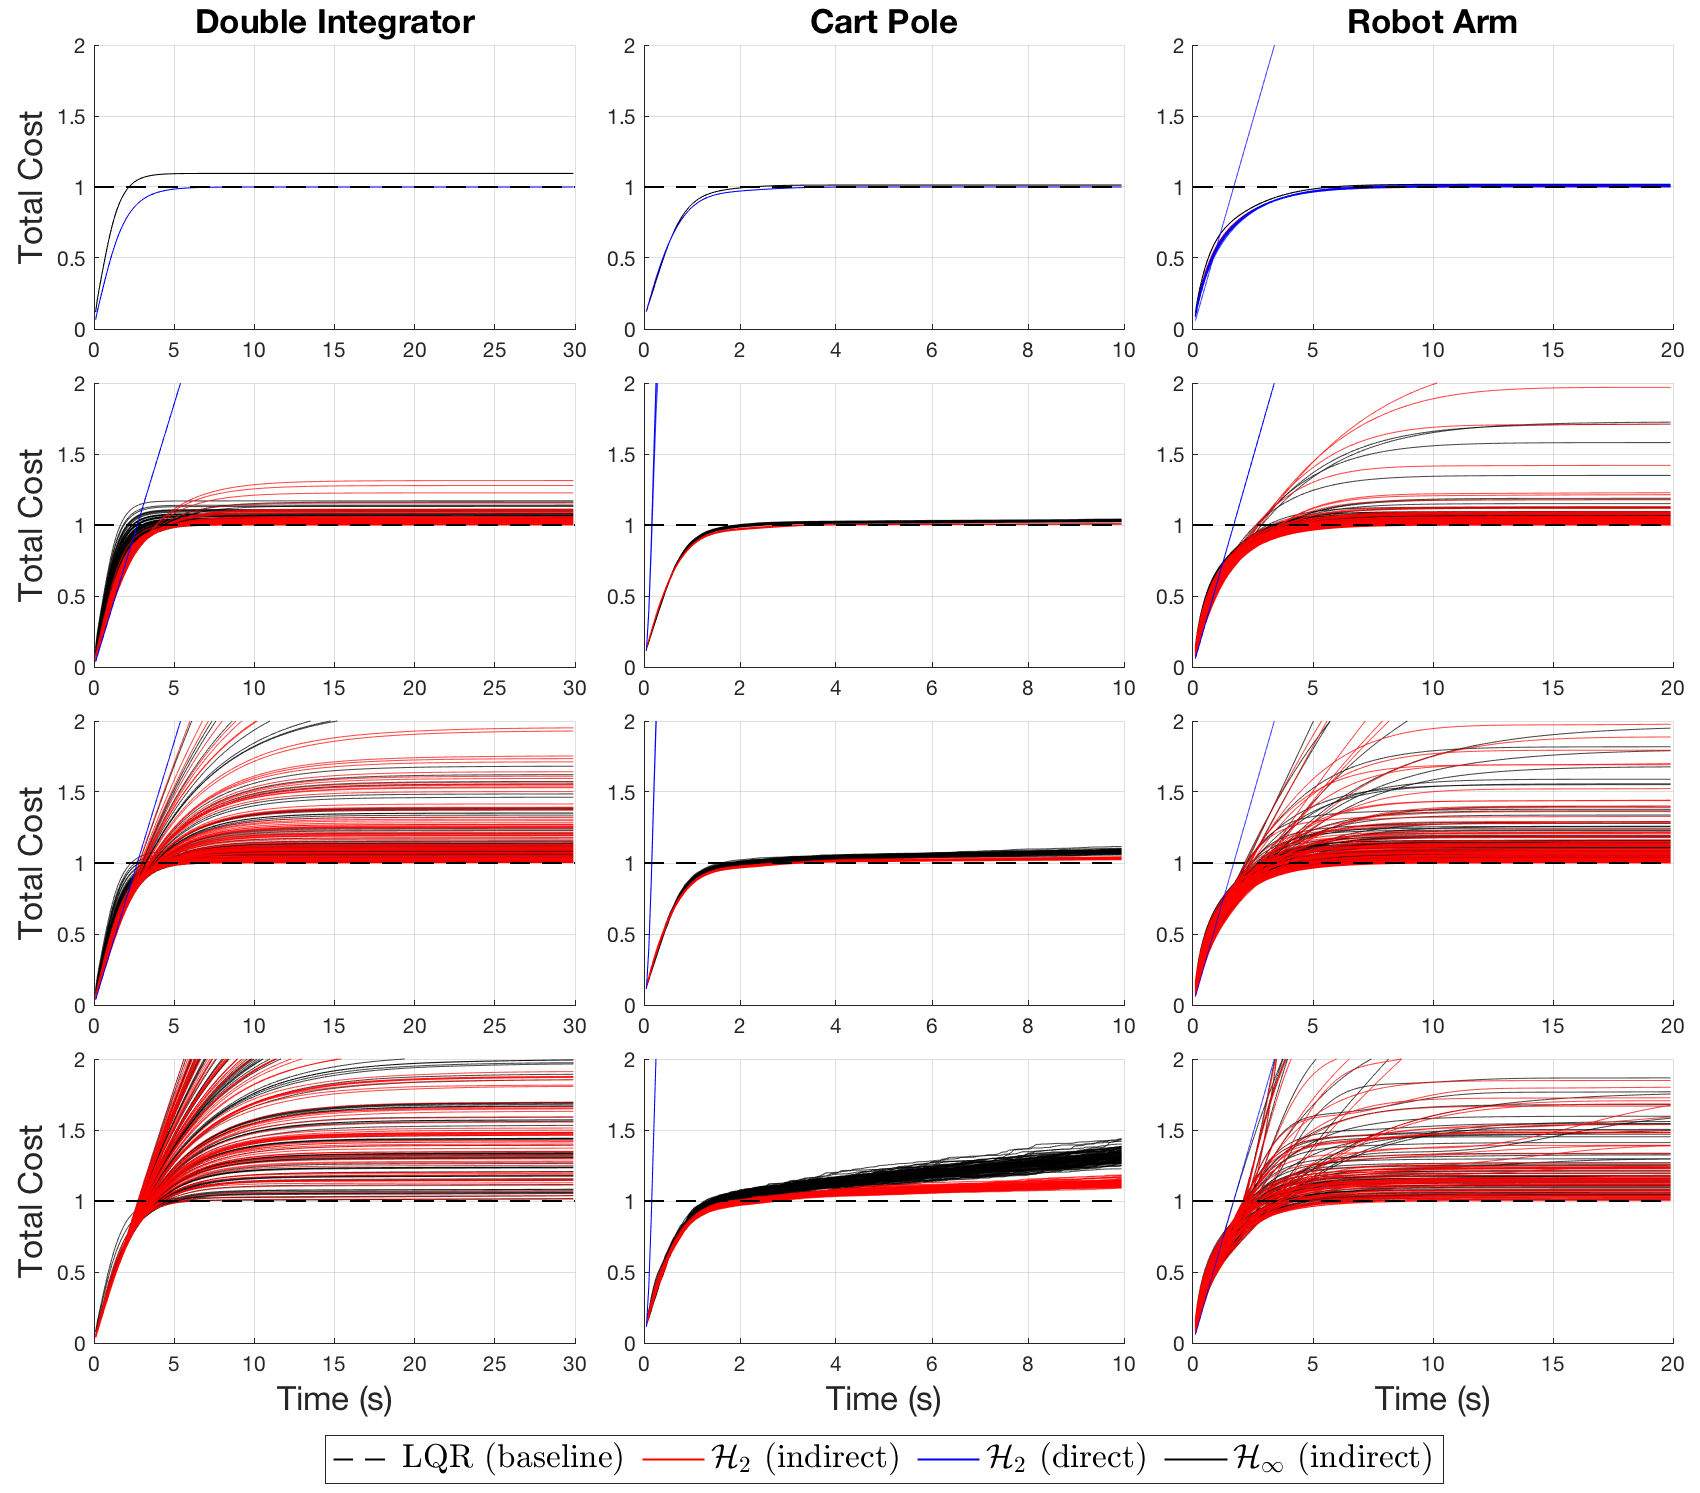
\includegraphics[width=\textwidth]{figures/noise_integrated_cost3.png}
\caption{Integrated LQ cost of the closed-loop generalized plant, for controllers learned from systems with measurement noise.  The rows correspond to respective scale factors of 0\%, 5\%, 10\%, and 20\%.  For each scale factor, the plots from 100 test runs are overlaid.}
\label{fig:noise_integrated_cost3}
\end{figure}

\newpage
\subsubsection{Overall Trends}
\underline{\textbf{Note}}: Averaged metrics shown in Figure \ref{fig:overall_trends_noise_opt_bar} are only defined for stable controllers, and may be skewed when the ``percent stable'' metric is significantly below 100\%.
\begin{figure}[H]
\centering
	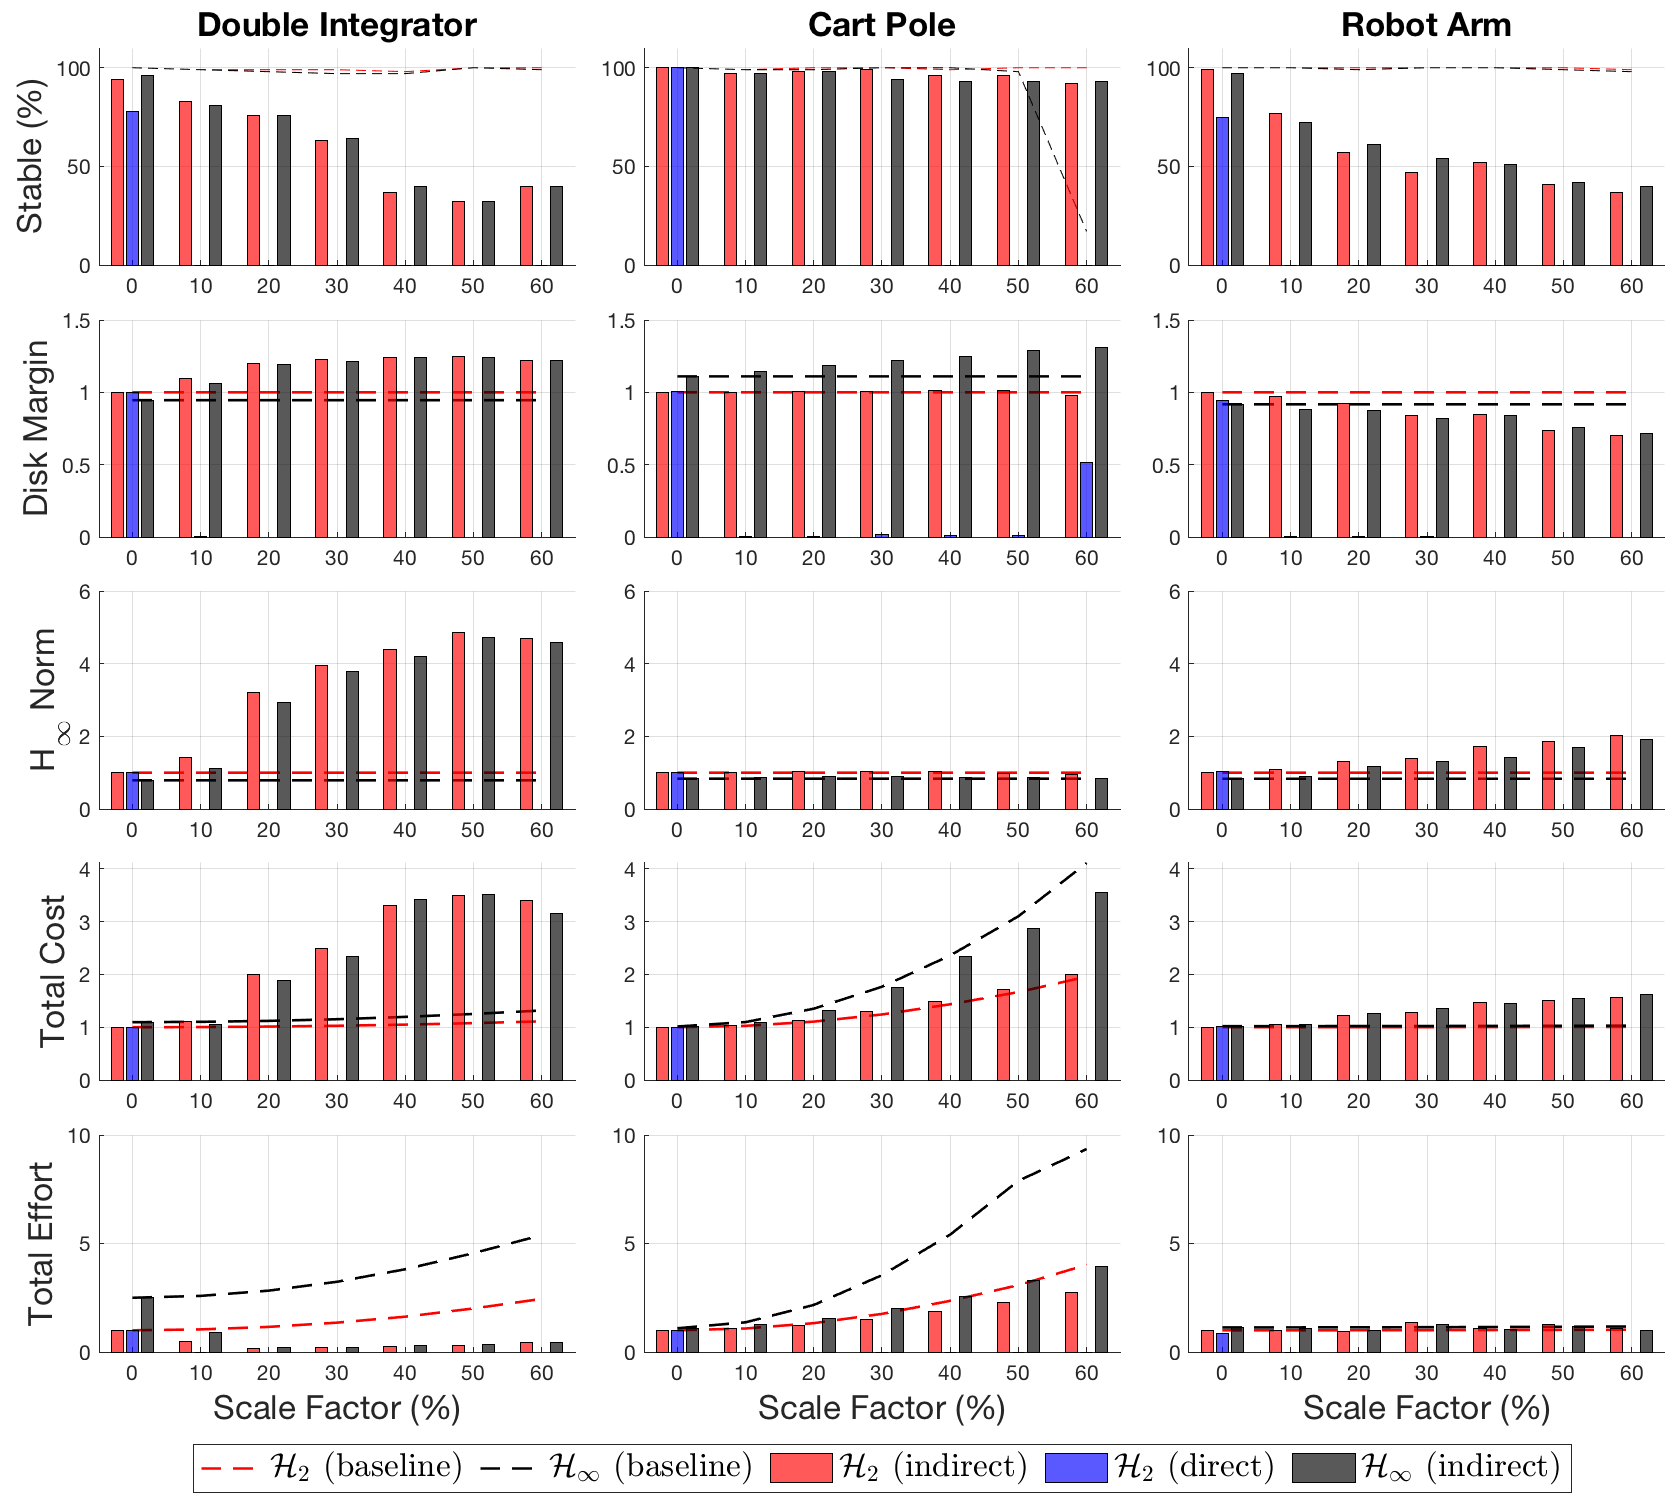
\includegraphics[width=\textwidth]{figures/overall_trends_noise_opt_bar.png}
\caption{Overall trends for scaled noise tests, comparing data-driven to baseline control approaches.  Apart from the percentage of stable controllers, all other metrics are normalized to what would be obtained by a nominal LQR/$\mathcal{H}_{2}$ feedback controller.  For each scale factor, the metrics shown are averaged across the stable test runs.}
\label{fig:overall_trends_noise_opt_bar}
\end{figure}

\newpage
\section{Test Results: Data-Driven Suboptimal $\mathcal{H}_{2}$ and $\mathcal{H}_{\infty}$}
\label{sect:results:data-driven-suboptimal}
These replace the $\mathcal{H}_{2}$-optimal LMI with the $\mathcal{H}_{2}$-suboptimal LMI described in Section \ref{sect:dataDrivenH2Suboptimal}.
\subsection{Parameter Uncertainty}
\subsubsection{Singular Values}
\begin{figure}[H]
\centering
	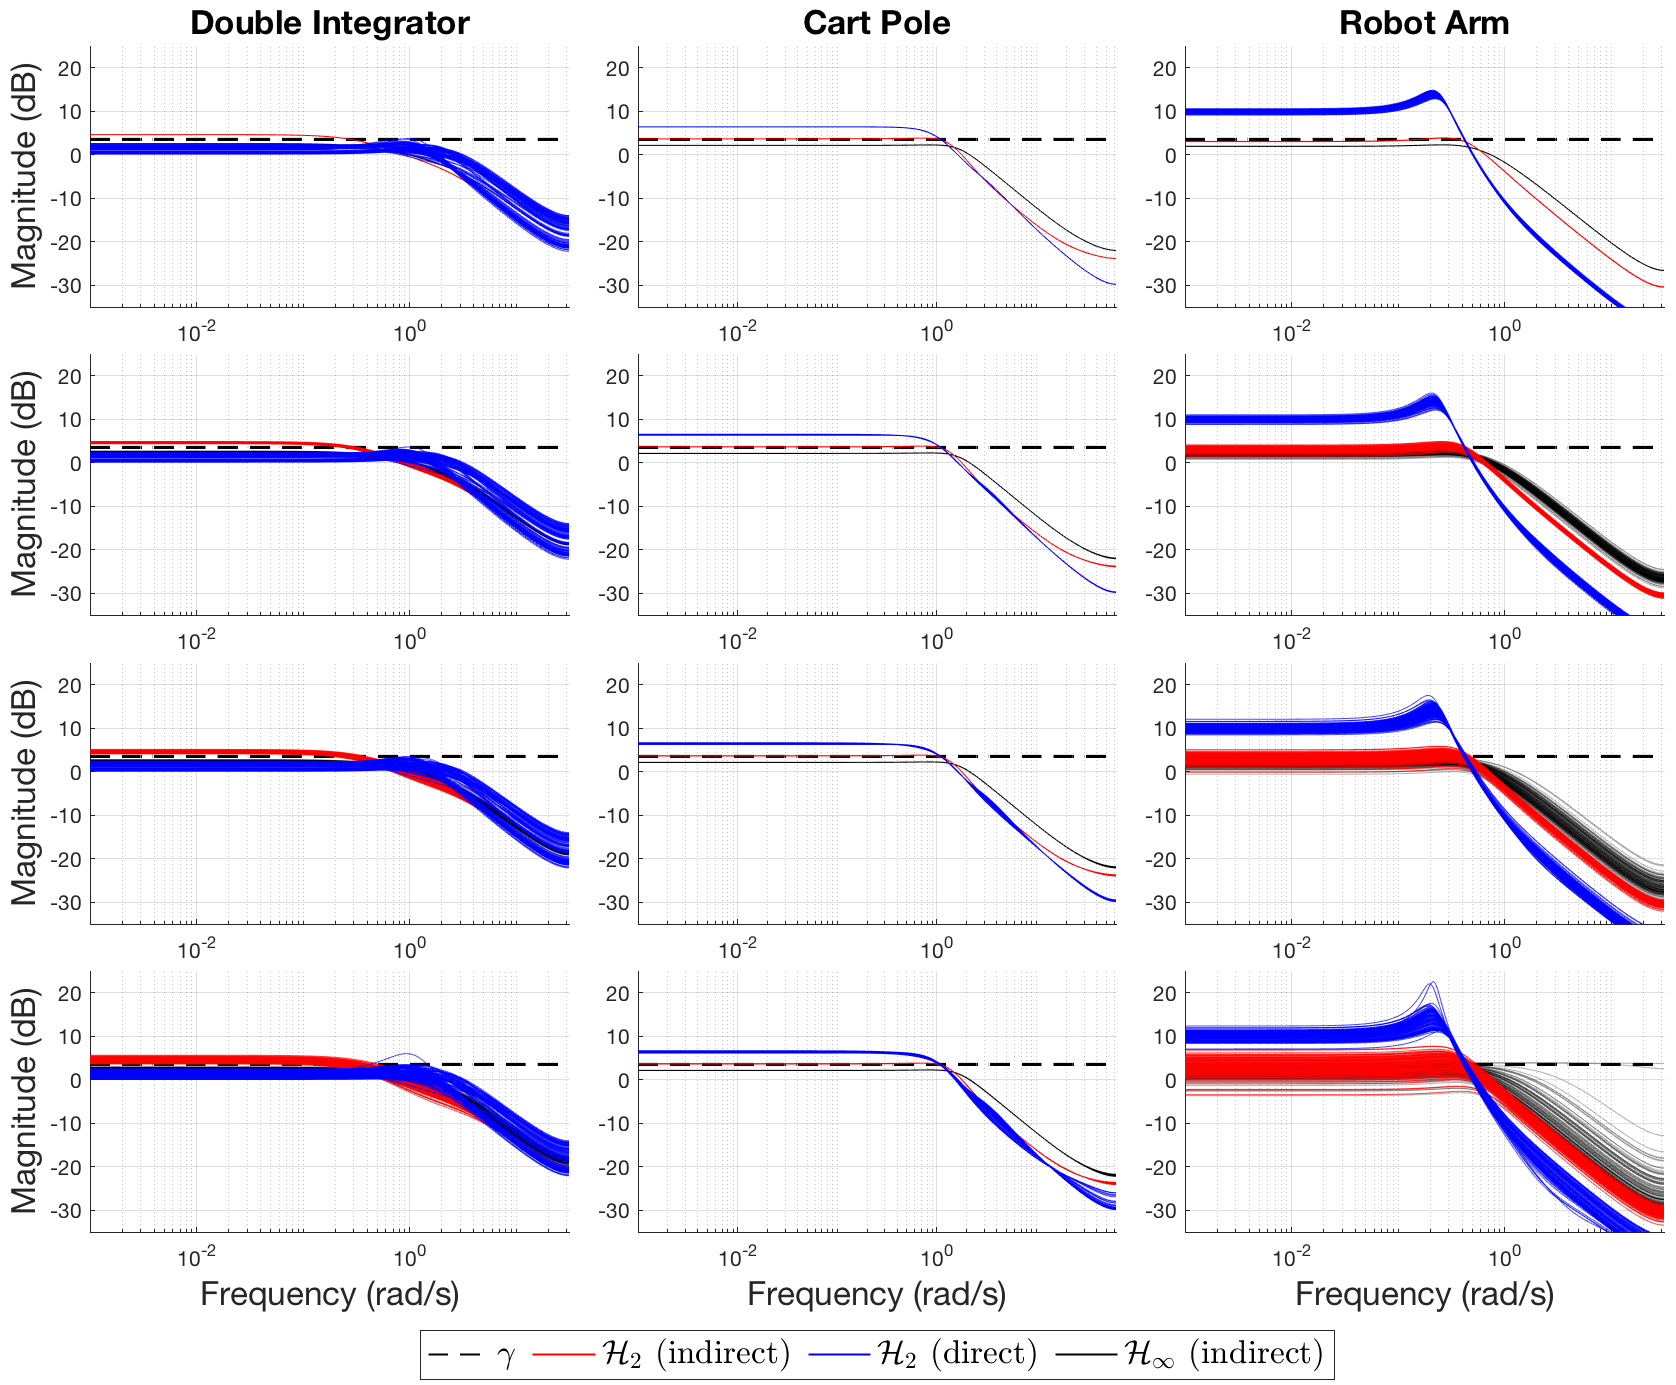
\includegraphics[width=\textwidth]{figures/uncertainty_singular_values4_s.png}
\caption{Maximum singular values of the closed-loop generalized plant, for controllers learned from systems with single-parameter uncertainty.  The rows correspond to respective scale factors of 0\%, 5\%, 10\%, and 20\%.  For each scale factor, the plots from 100 test runs are overlaid.}
\label{fig:uncertainty_singular_values4_s}
\end{figure}

\newpage
\subsubsection{Integrated Control Effort}
\begin{figure}[H]
\centering
	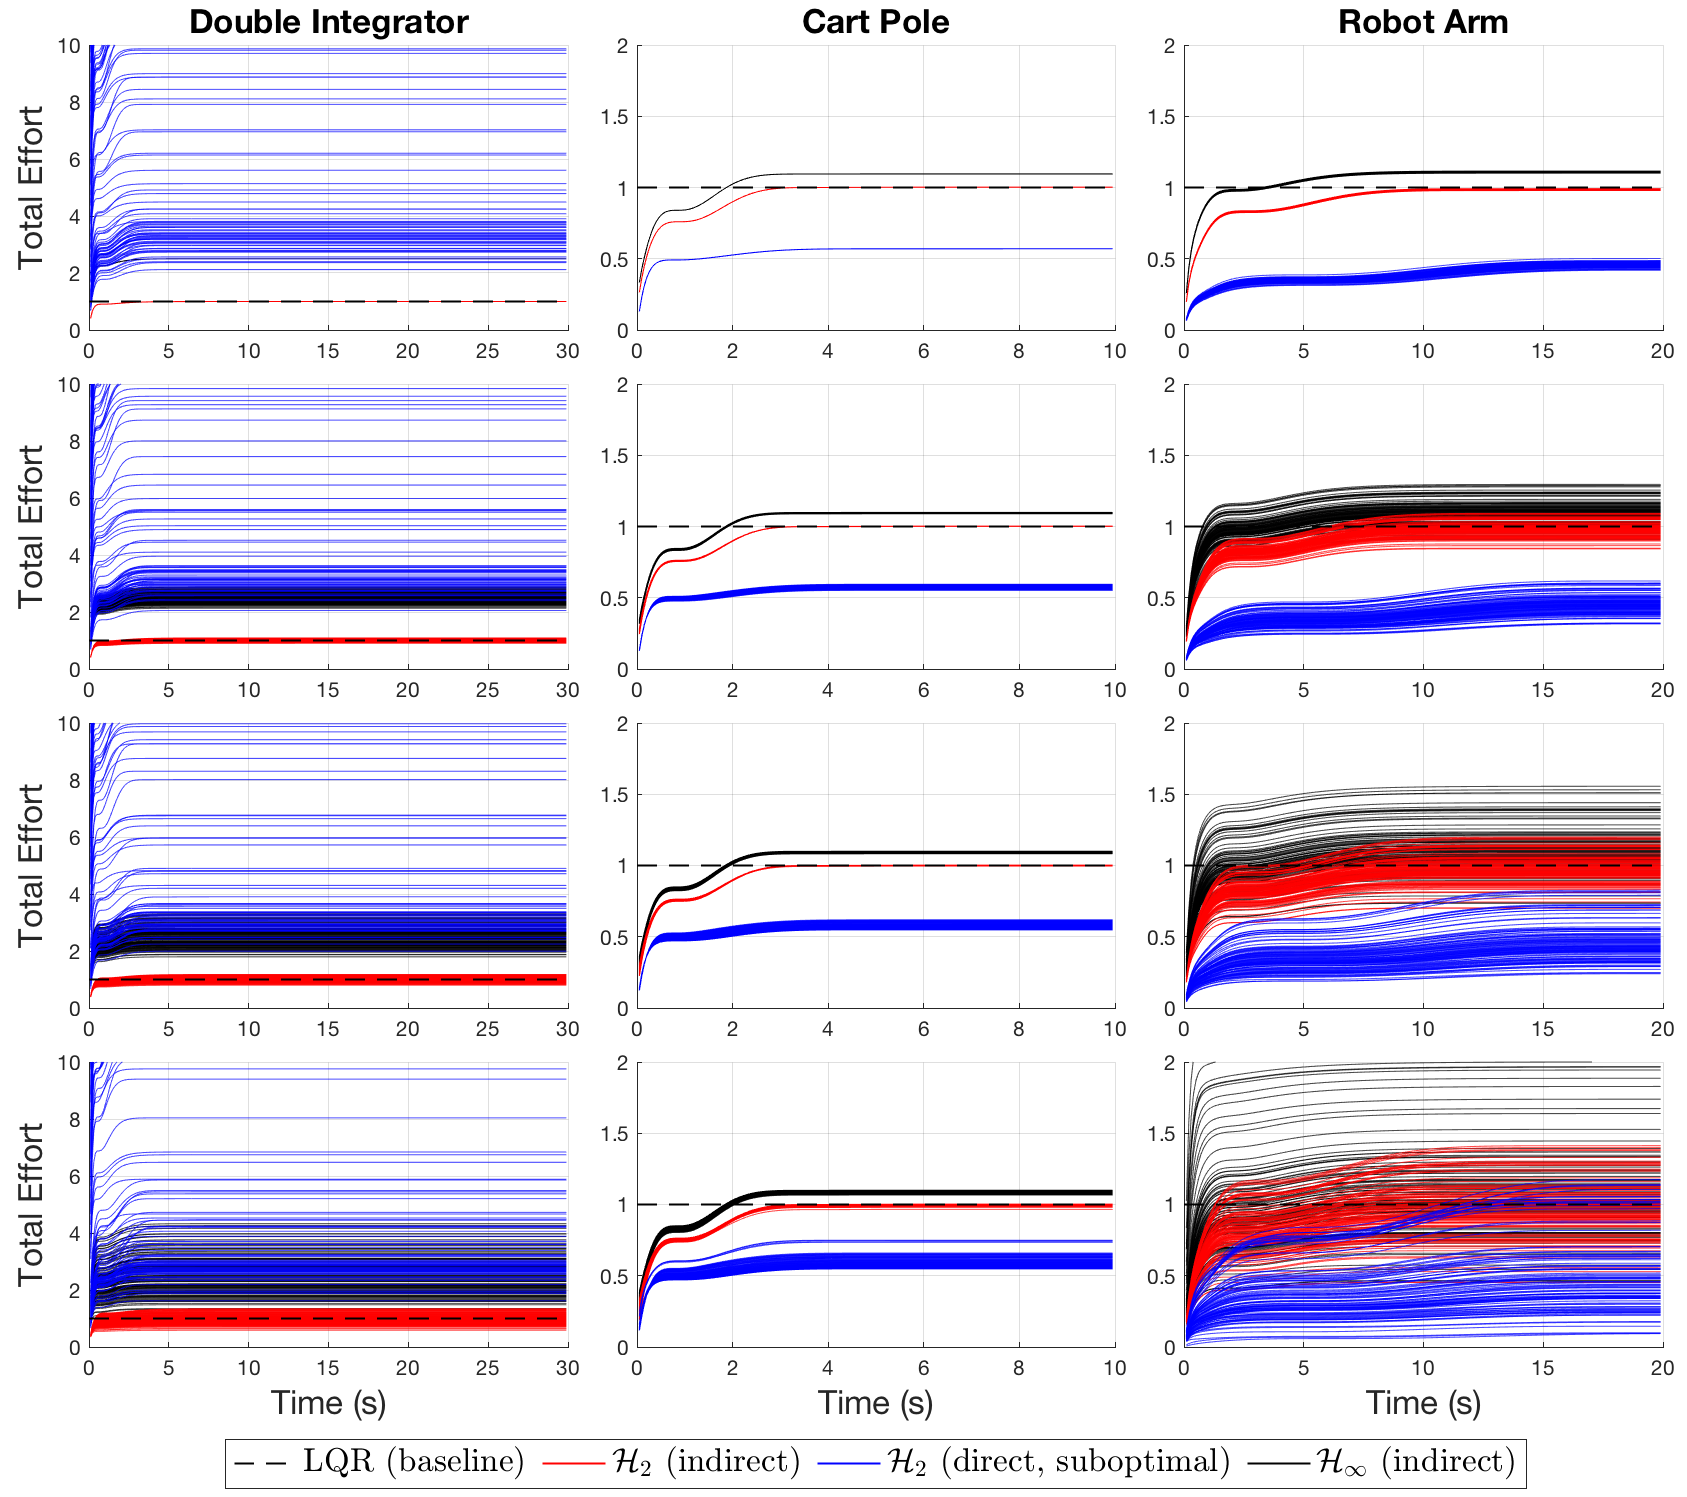
\includegraphics[width=\textwidth]{figures/uncertainty_integrated_effort4_s.png}
\caption{Integrated control effort of the closed-loop generalized plant, for controllers learned from systems with single-parameter uncertainty.  The rows correspond to respective scale factors of 0\%, 5\%, 10\%, and 20\%.  For each scale factor, the plots from 100 test runs are overlaid.}
\label{fig:uncertainty_integrated_effort4_s}
\end{figure}

\newpage
\subsubsection{Integrated LQ Cost}
\begin{figure}[H]
\centering
	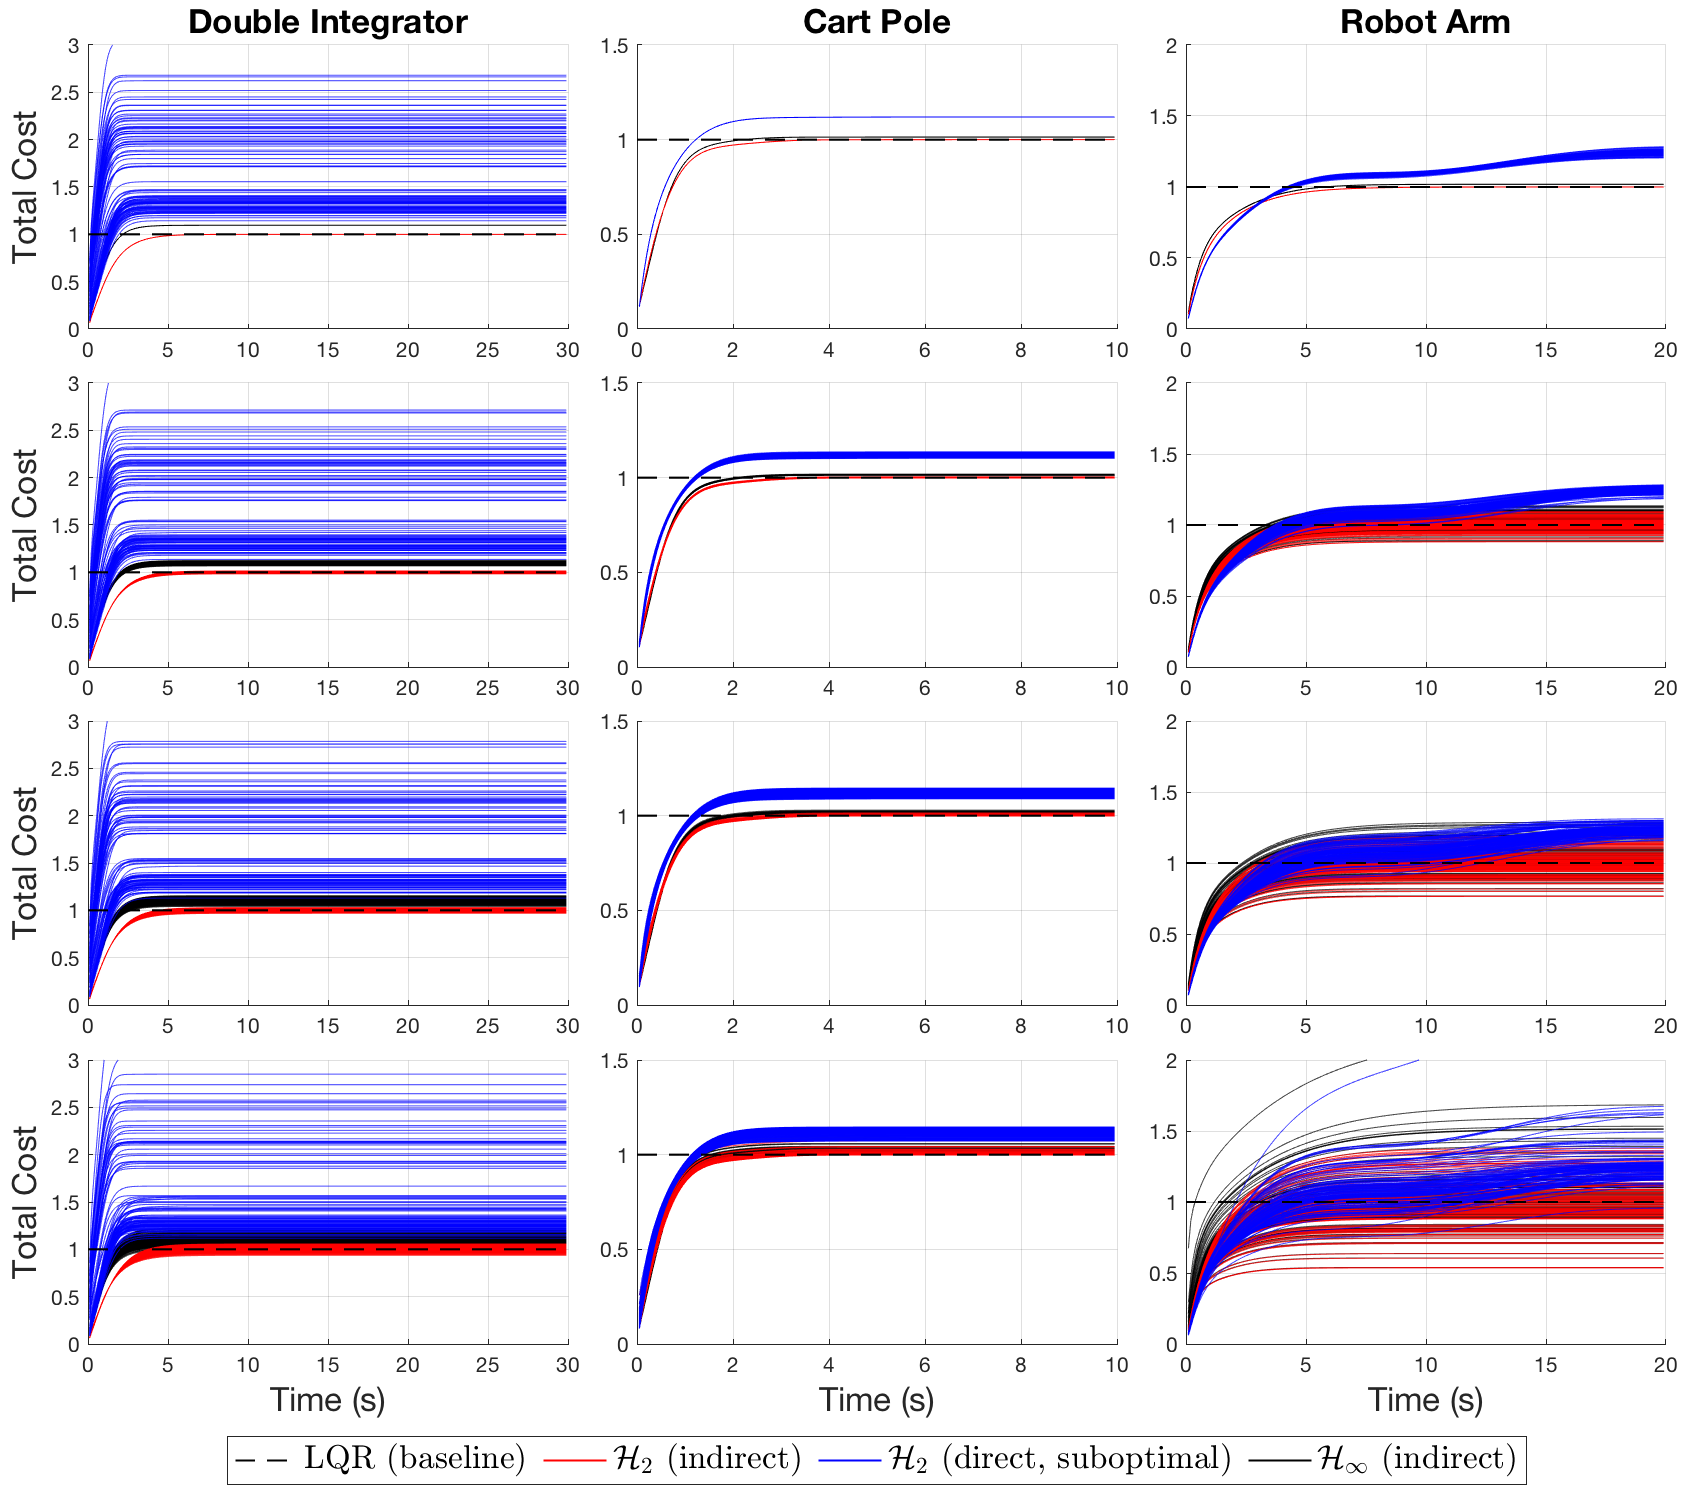
\includegraphics[width=\textwidth]{figures/uncertainty_integrated_cost4_s.png}
\caption{Integrated LQ cost of the closed-loop generalized plant, for controllers learned from systems with single-parameter uncertainty.  The rows correspond to respective scale factors of 0\%, 5\%, 10\%, and 20\%.  For each scale factor, the plots from 100 test runs are overlaid.}
\label{fig:uncertainty_integrated_cost4_s}
\end{figure}

\newpage
\subsubsection{Overall Trends}
\underline{\textbf{Note}}: Averaged metrics shown in Figure \ref{fig:overall_trends_uncertainty_subopt_bar} are only defined for stable controllers, and may be skewed when the ``percent stable'' metric is significantly below 100\%.
\begin{figure}[H]
\centering
	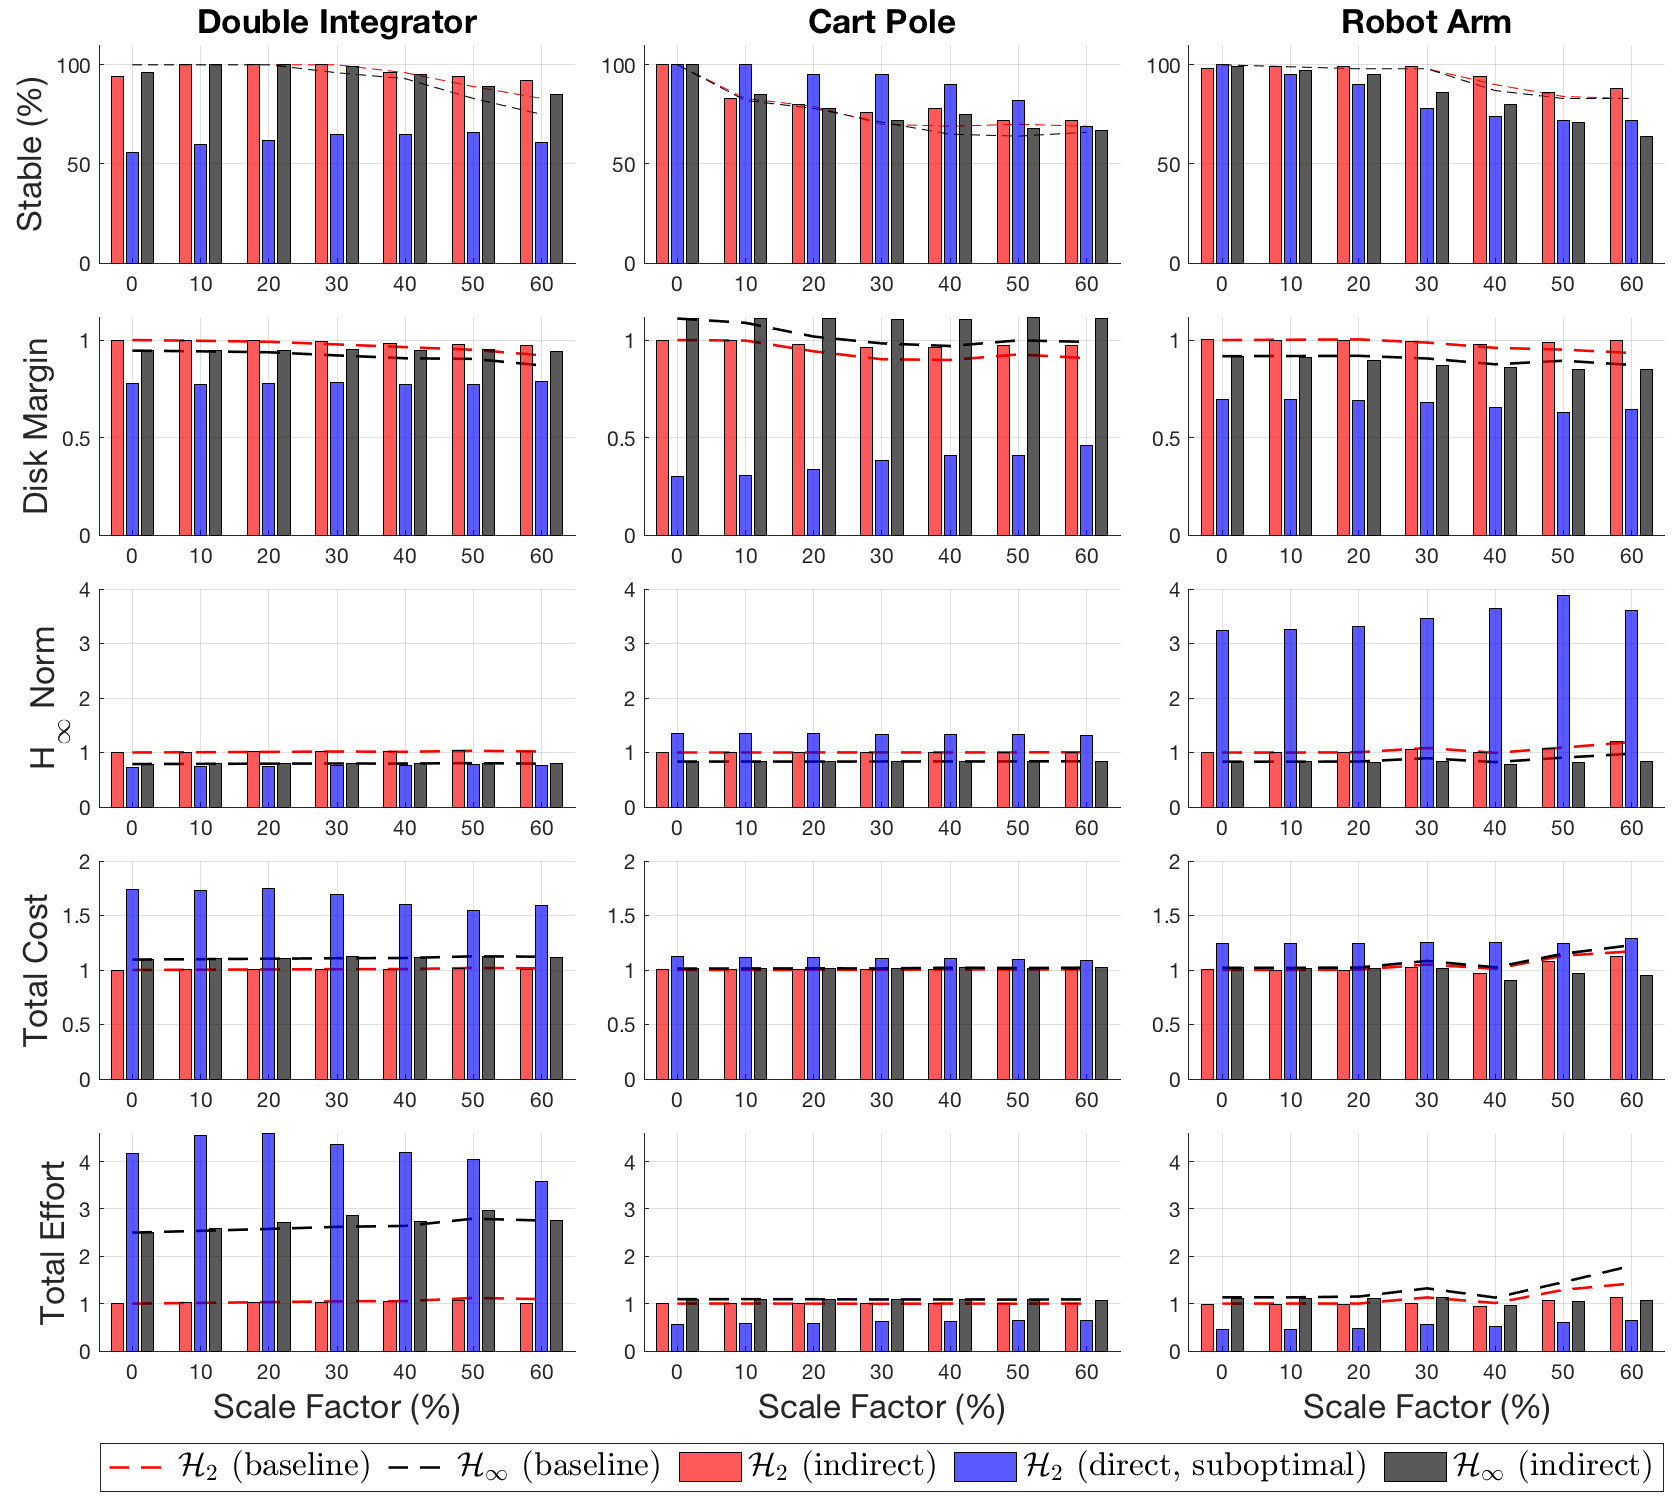
\includegraphics[width=\textwidth]{figures/overall_trends_uncertainty_subopt_bar.png}
\caption{Overall trends for scaled uncertainty tests, comparing data-driven to baseline control approaches.  Apart from the percentage of stable controllers, all other metrics are normalized to what would be obtained by a nominal LQR/$\mathcal{H}_{2}$ feedback controller.  For each scale factor, the metrics shown are averaged across the stable test runs.}
\label{fig:overall_trends_uncertainty_subopt_bar}
\end{figure}

\newpage
\subsection{Measurement Noise}
\subsubsection{Singular Values}
\begin{figure}[H]
\centering
	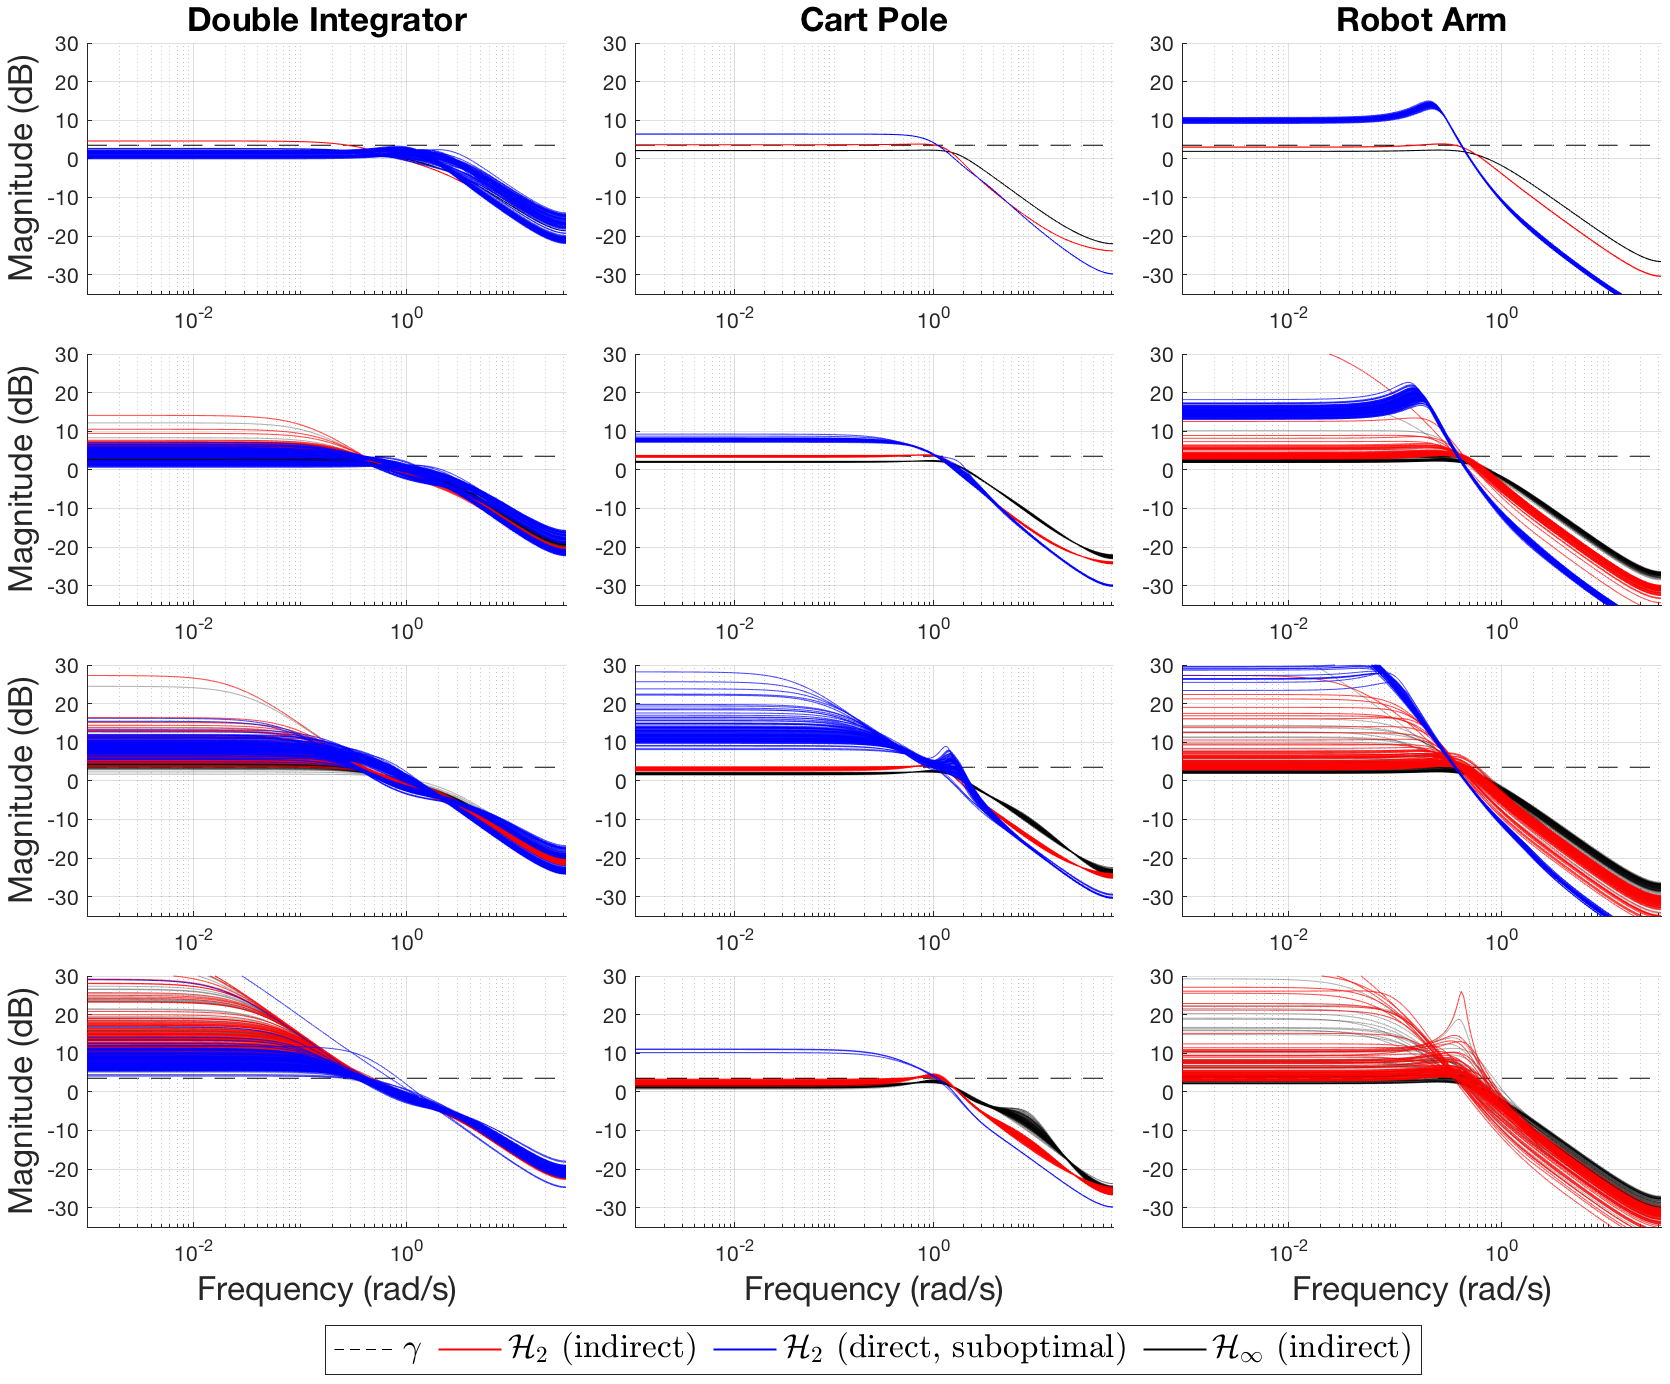
\includegraphics[width=\textwidth]{figures/noise_singular_values4_s.png}
\caption{Maximum singular values of the closed-loop generalized plant, for controllers learned from systems with measurement noise.  The rows correspond to respective scale factors of 0\%, 5\%, 10\%, and 20\%.  For each scale factor, the plots from 100 test runs are overlaid.}
\label{fig:noise_singular_values4_s}
\end{figure}

\newpage
\subsubsection{Integrated Control Effort}
\begin{figure}[H]
\centering
	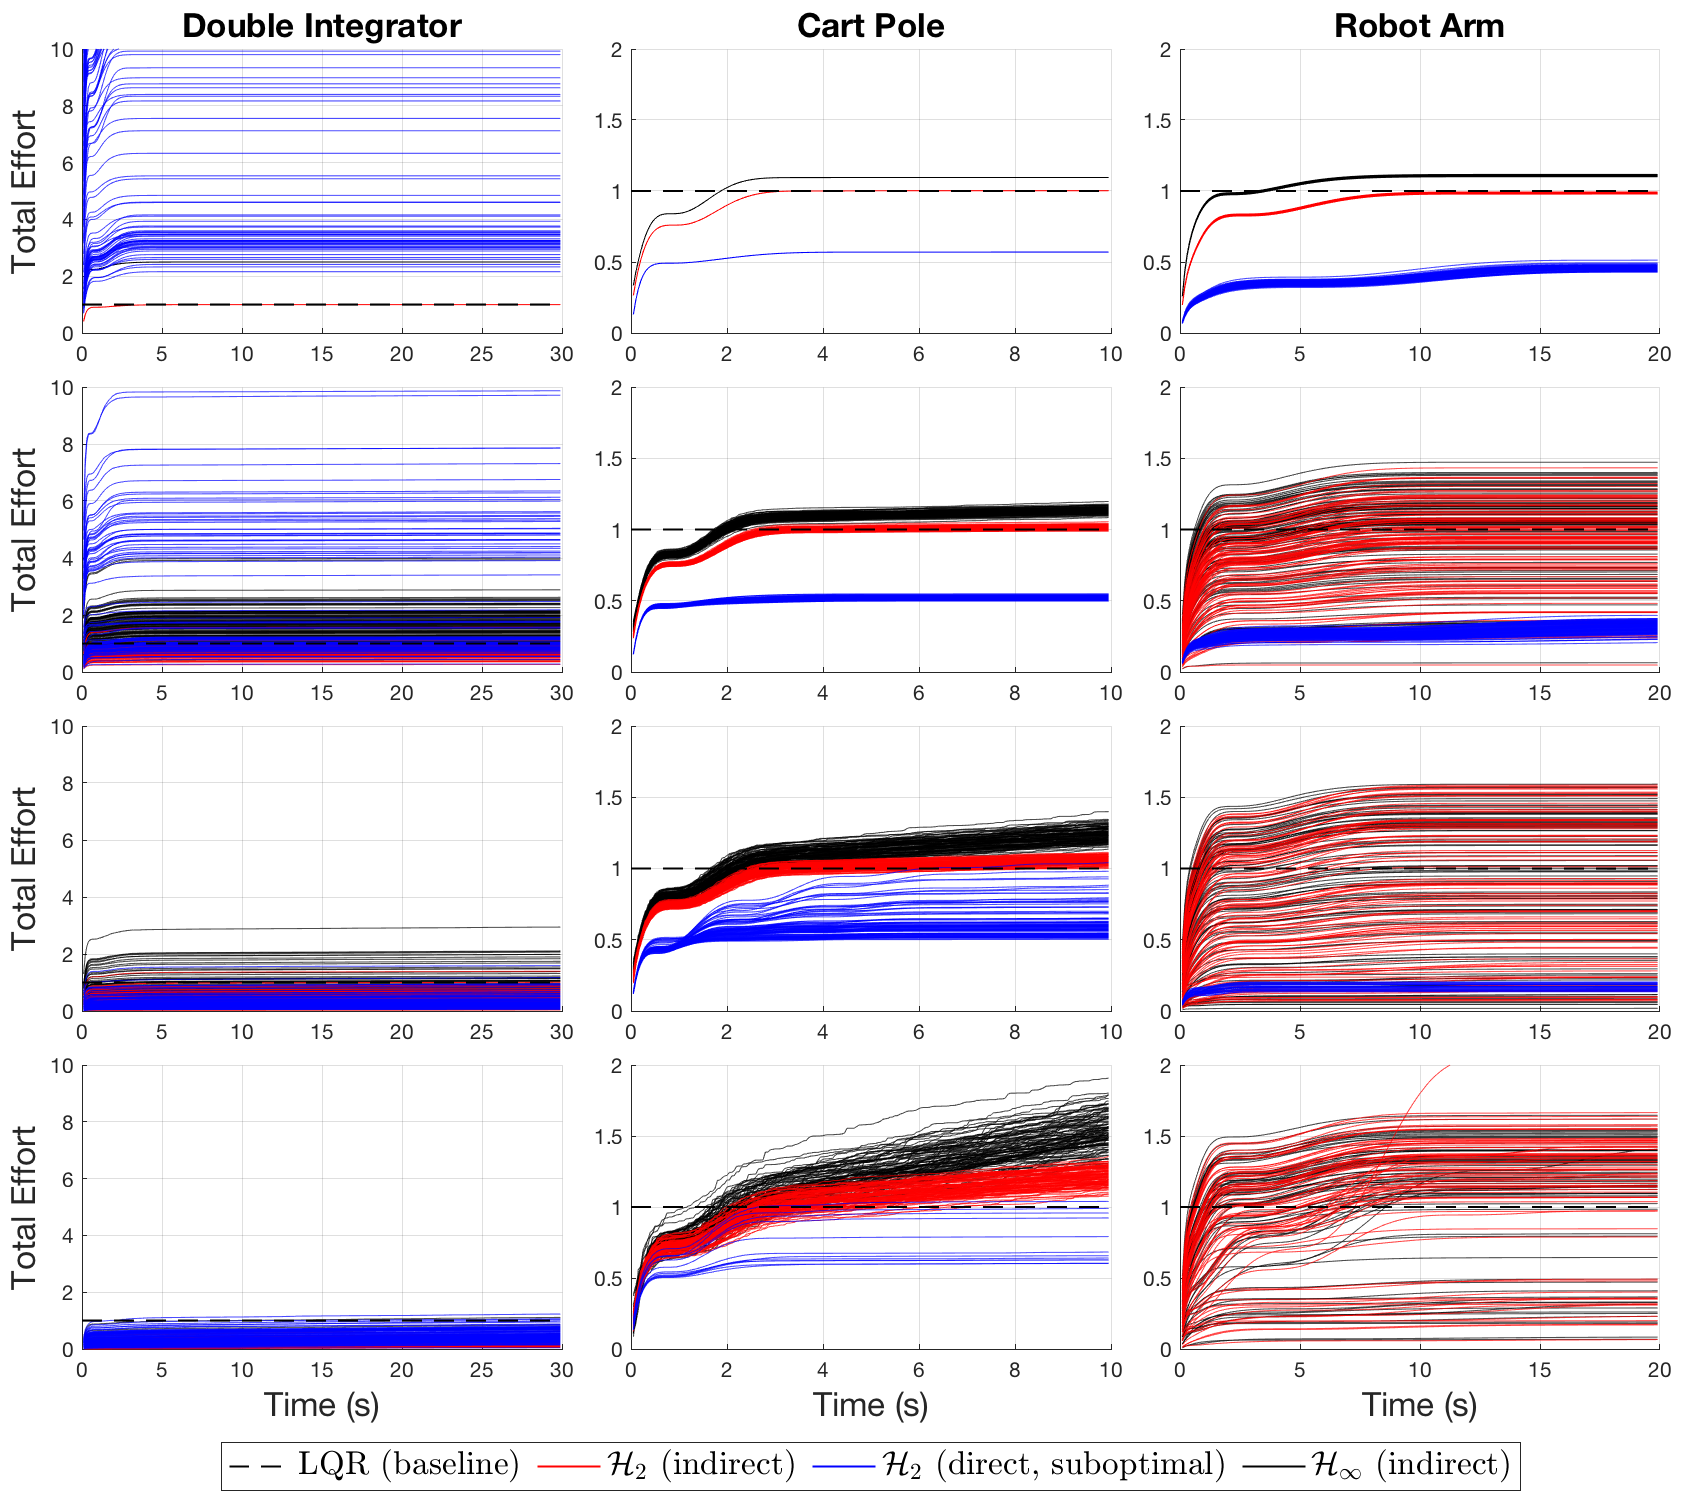
\includegraphics[width=\textwidth]{figures/noise_integrated_effort4_s.png}
\caption{Integrated control effort of the closed-loop generalized plant, for controllers learned from systems with measurement noise.  The rows correspond to respective scale factors of 0\%, 5\%, 10\%, and 20\%.  For each scale factor, the plots from 100 test runs are overlaid.}
\label{fig:noise_integrated_effort4_s}
\end{figure}

\newpage
\subsubsection{Integrated LQ Cost}
\begin{figure}[H]
\centering
	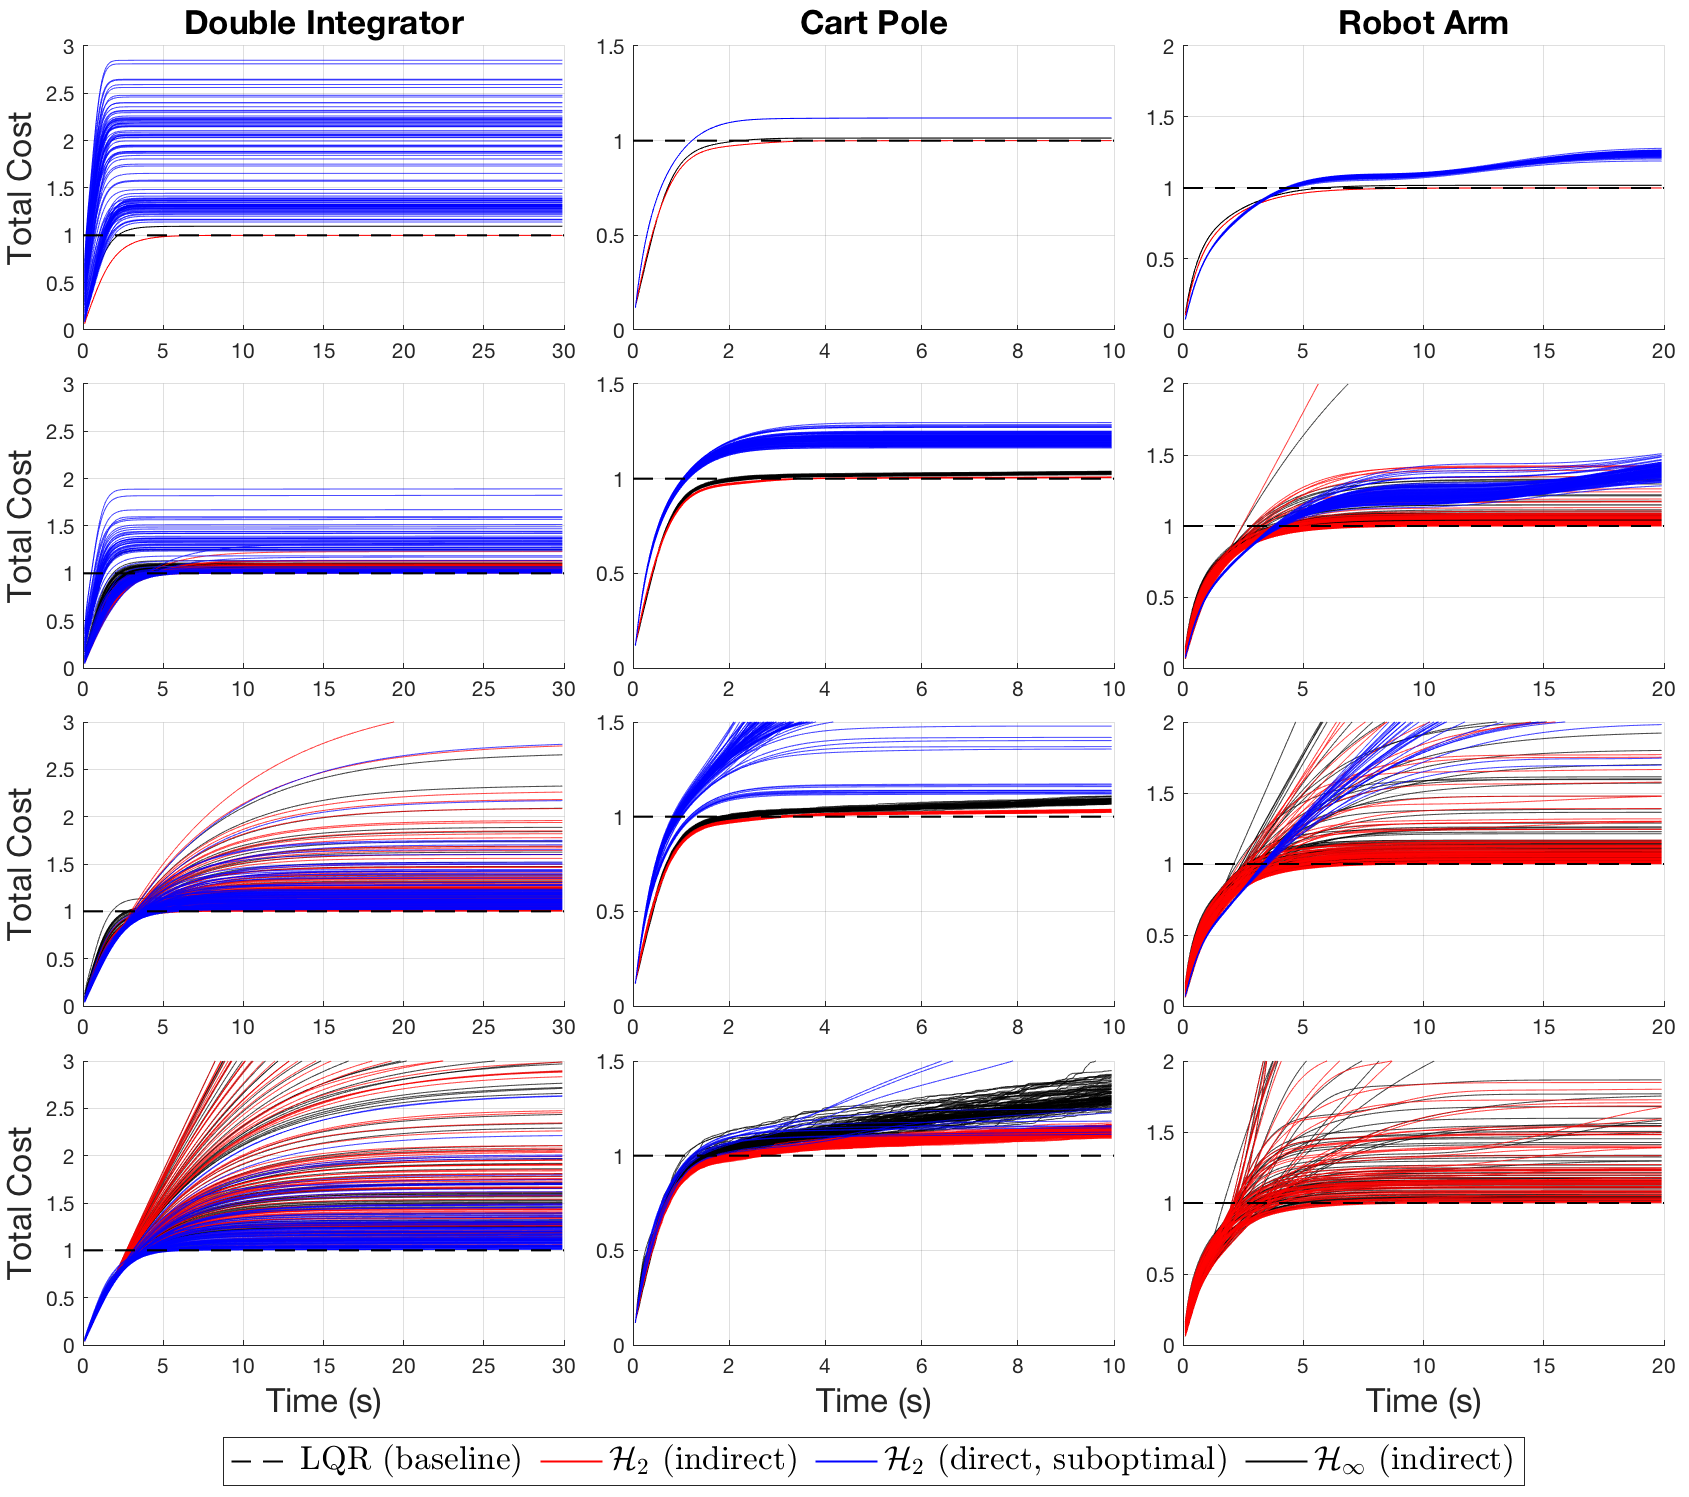
\includegraphics[width=\textwidth]{figures/noise_integrated_cost4_s.png}
\caption{Integrated LQ cost of the closed-loop generalized plant, for controllers learned from systems with measurement noise.  The rows correspond to respective scale factors of 0\%, 5\%, 10\%, and 20\%.  For each scale factor, the plots from 100 test runs are overlaid.}
\label{fig:noise_integrated_cost4_s}
\end{figure}

\newpage
\subsubsection{Overall Trends}
\underline{\textbf{Note}}: Averaged metrics shown in Figure \ref{fig:overall_trends_noise_subopt_bar} are only defined for stable controllers, and may be skewed when the ``percent stable'' metric is significantly below 100\%.
\begin{figure}[H]
\centering
	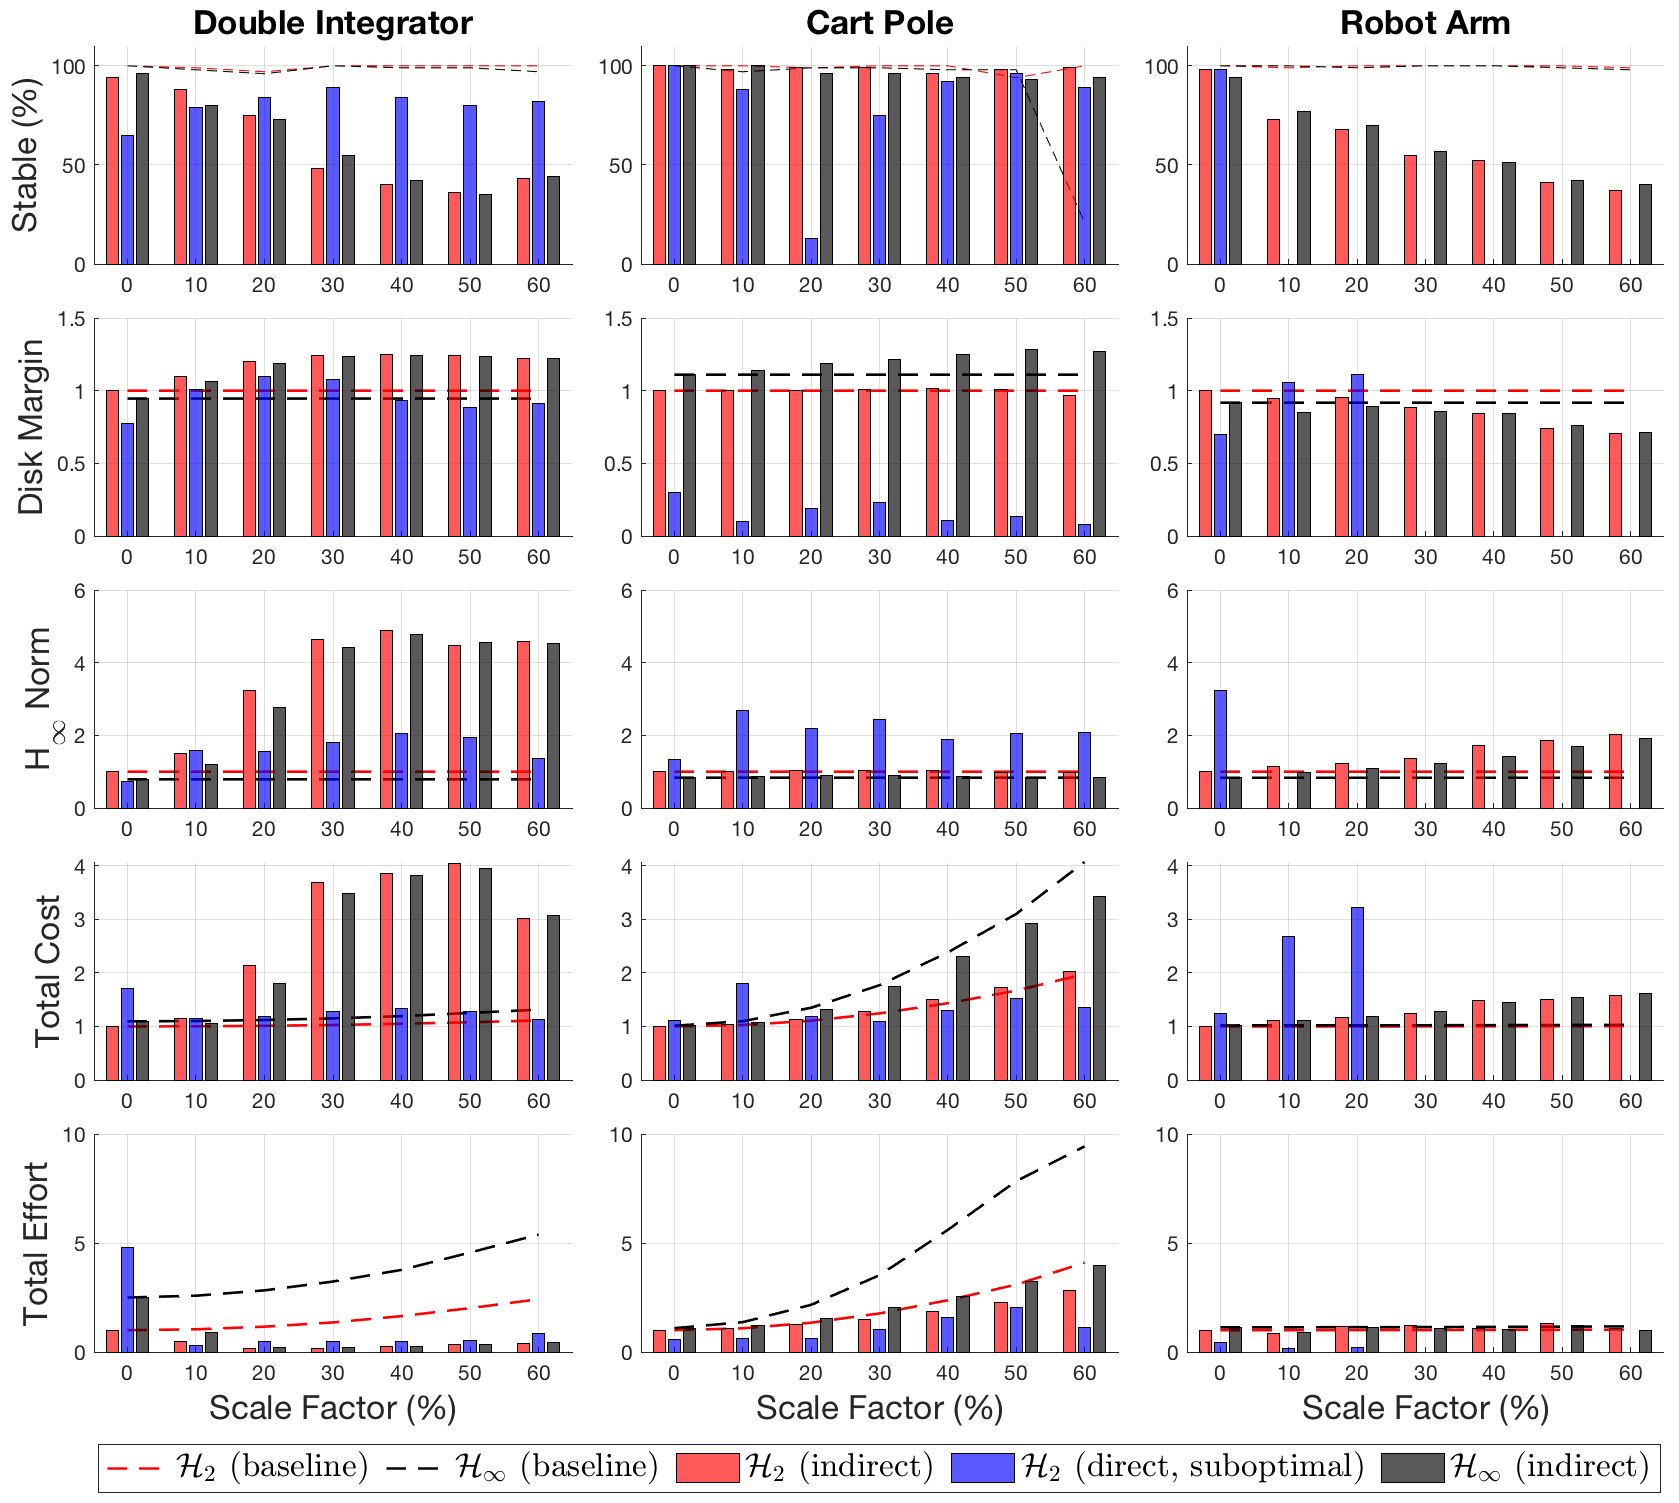
\includegraphics[width=\textwidth]{figures/overall_trends_noise_subopt_bar.png}
\caption{Overall trends for scaled noise tests, comparing data-driven to baseline control approaches.  Apart from the percentage of stable controllers, all other metrics are normalized to what would be obtained by a nominal LQR/$\mathcal{H}_{2}$ feedback controller.  For each scale factor, the metrics shown are averaged across the stable test runs.}
\label{fig:overall_trends_noise_subopt_bar}
\end{figure}

\section{Discussion}
\label{sect:results:discussion}
\subsection{Effect of Parameter Uncertainty}
Figures \ref{fig:uncertainty_singular_values3}, \ref{fig:uncertainty_integrated_effort3}, \ref{fig:uncertainty_integrated_cost3} and \ref{fig:overall_trends_uncertainty_opt_bar} illustrate the data-driven control techniques when parameter uncertainty is present (both in training data and simulation).  The variation in parameter uncertainty produced variation in all metrics.  In terms of singular values, the general loop shape was preserved, although as the uncertainty's variance was increased, the maximum singular values at higher frequencies were varied.  Note that in Figure \ref{fig:uncertainty_singular_values3}, the dotted black line represents the $\mathcal{H}_{\infty}$-optimal disturbance attenuation gain.  The $\mathcal{H}_{2}$ controllers are expected to be slightly above this line, and the $\mathcal{H}_{\infty}$ controllers are expected to be at or below it.  For the robot arm in particular, direct data-driven $\mathcal{H}_{2}$ control produced several marginally stable controllers, even for the nominal model, and this occurred more frequently as the scale factor was increased.

Note that in Figures \ref{fig:uncertainty_integrated_effort3} and \ref{fig:uncertainty_integrated_cost3}, the total cost and effort are scaled by the infinite-horizon LQR cost achieved without parameter uncertainty or noise.  The $\mathcal{H}_{2}$ controllers are expected to achieve this performance exactly, and the $\mathcal{H}_{\infty}$ control performance depends on the plant model (see Figure \ref{fig:baseline_integrated_cost}).  From these figures, the cart pole's performance is degraded far less than the double integrator and robot arm, which both see increased variation spreading roughly 5-10 times higher.  Arguably, these both have much more oversimplified dynamic models, which likely makes data-driven control more sensitive due to the lesser contribution of internal state dynamics to the overall input/output data observed in a particular set of training data.

Figure \ref{fig:overall_trends_uncertainty_opt_bar} illustrates the overall trends for this test.  Note that rows 2-5 are normalized to the baseline LQR control, and are thus not absolute.  These should be interpreted as the performance of the data-driven approaches relative to the LQ optimal regulator on a system without uncertainty.

In terms of the fraction of stabilizing controllers (per 100 runs), all data-driven methods saw a decrease from 100\% down to 80\% or less as the scale factor increased.  Note that the dotted ``baseline'' lines also trend downward because the baseline controllers (when applied to the full system) eventually reach a point where nominal performance is lost due to the effect of model uncertainty.

The remaining metrics are relatively constant, though it should be noted once again these are only computed for the fraction of controllers which are stable.  What can be said is that, for those which were stable, the robustness metrics were relatively constant despite higher uncertainty.  This could be due to the training data not providing enough information to adequately characterize the off-nominal system.  Because the training policy was held constant across all tests, there could conceivably be a shift in plant dynamics which is effectively unaccounted for during training.

\subsection{Effect of Measurement Noise}
Figures \ref{fig:noise_singular_values3}, \ref{fig:noise_integrated_effort3}, \ref{fig:noise_integrated_cost3} and \ref{fig:overall_trends_noise_opt_bar} illustrate the data-driven control techniques when measurement noise is present (both in training data and simulation).  Figures \ref{fig:noise_integrated_effort3} and \ref{fig:noise_integrated_cost3} illustrate the effect of measurement noise on the integrated performance.  Overall trends are shown in Figure \ref{fig:overall_trends_noise_opt_bar}.

In all of the plots, it is clear that the direct (LMI-based) data-driven approach did not work when the scale factor was above 10\%.  This is due to the specification of the optimization problem, which does not account for any perturbation in the data matrices.  The indirect (SVD-based) approaches do work somewhat, though their success rate is less than 100\% and trends downward significantly for both double integrator and robot arm.  The fact that the cart pole sees adequate performance from indirect data-driven control is partly due to the fact its input/output data has more information from the state dynamics than the other two systems (a pattern also seen in Figure \ref{fig:overall_trends_uncertainty_opt_bar}).  This also highlights a relative merit of indirect data-driven control: unlike the LMI-based algorithm, the SVD provides some inherent robustness to uncorrelated noise, if the system modes are able to be observed in the training data.

In examining integrated metrics, it should be noted that increasing the scale factor is expected to cause a rise in final cost/effort.  Even after stabilization, the system continues to respond to noise in the feedback loop.  If the total cost was instead averaged over a long enough horizon (to estimate its infinite-horizon expected value), one would expect a decay.

\subsection{Effect of Performance Objective}
Numerical results also differ when directly-learned $\mathcal{H}_{2}$ controllers optimize a performance objective which allows some slack.  This was hypothesized to have some impact on how effective data-driven control was when uncertainty or noise was present (both in training data and regular plant operation).  To examine the effect of a suboptimal performance objective, the same scaled uncertainty/noise tests were run, but instead of solving the direct $\mathcal{H}_{2}$ control LMI given by Equation \eqref{eq:h2_lmi_dd}, the suboptimal variant given by Equation \eqref{eq:h2s_lmi_dd} was used instead.  Results for parameter uncertainty are plotted in Figures \ref{fig:uncertainty_singular_values4_s}, \ref{fig:uncertainty_integrated_effort4_s}, \ref{fig:uncertainty_integrated_cost4_s}, and \ref{fig:overall_trends_uncertainty_subopt_bar} and results for measurement noise are plotted in Figures \ref{fig:noise_singular_values4_s}, \ref{fig:noise_integrated_effort4_s}, \ref{fig:noise_integrated_cost4_s}, and \ref{fig:overall_trends_noise_opt_bar}.

When subjected to scaled parameter uncertainty, the suboptimal $\mathcal{H}_{2}$ technique did produce more stable controllers than the optimal $\mathcal{H}_{2}$ technique.  However, between the two, the suboptimal versions consistently showed lower stability margins, higher $\mathcal{H}_{\infty}$ norms, and higher integrated effort/LQ cost.

It is interesting to note the control effort used by the direct approach for cart pole and robot arm are on average half of what is used by the baseline and indirectly learned controllers, while the overall LQ cost is higher (10-15\% for the cart pole, and about 20-30\% for the robot arm).  This is a result of the suboptimal control objective, which effectively causes a different relative weighting between state error and control effort.  It would be interesting to investigate other choices of LQ cost weights $\vb*{Q}_{x}$ and $\vb*{R}_{u}$ which produce similar baseline performance to see whether the data-driven approach more easily finds the optimum.
